
\begin{appendix}
\onecolumn

\tableofcontents
\clearpage

\section{Contributions}
Names ordered alphabetically.

\paragraph{Model training and experiment babysitting.} Achal Dave (notably, the 1.4B parameter, 900B token run),
Samir Yitzhak Gadre

\paragraph{Dataloading.}
Georgios Smyrnis

\paragraph{Training tokens.} Achal Dave, Alex Fang, Samir Yitzhak Gadre, Suchin Gururangan, Jeffrey Li, Vaishaal Shankar (lead), Mitchell Wortsman

\paragraph{Evaluation tokens.} Achal Dave, Samir Yitzhak Gadre, Reinhard Heckel, Vaishaal Shankar (lead), Rulin Shao

\paragraph{Loss/perplexity evaluation.} Samir Yitzhak Gadre
\paragraph{Downstream evaluation.} Vaishaal Shankar

\paragraph{Project-specific planning, infrastructure, plots, and analysis.}
Samir Yitzhak Gadre

\paragraph{OpenLM~\cite{open_lm} open-source infrastructure.}
Achal Dave (core contributor),
Alex Fang,
Samir Yitzhak Gadre (core contributor),
Suchin Gururangan (core contributor),
Jenia Jitsev,
Sedrick Keh,
Jeffrey Li,
Jean Mercat,
Marianna Nezhurina,
Vaishaal Shankar (core contributor),
Georgios Smyrnis (core contributor),
Igor Vasiljevic,
Mitchell Wortsman (core contributor),
Rui Xin


\paragraph{Theory.}
Yair Carmon (original idea that ``parallel lines'' should show up in scaling plots),
Samir Yitzhak Gadre (various derivations, empirical verification, related validation loss to average top-1 error as in Equation~\eqref{eq:errL}),
Reinhard Heckel (derived a scaling form based on Chinchilla~Approach~3~\cite{chinchilla}, which appears in Equation~\eqref{eq:lossCM}),
Niklas Muennighoff (derived a scaling form based on Chinchilla Approach~3, similar to Equation~\eqref{eq:lossCM}),
Mitchell Wortsman (provided intuition about irreducible loss and why it is critical).

\paragraph{Writing.}
Yair Carmon,
Achal Dave,
Reinhard Heckel,
Samir Yitzhak Gadre (lead), 
Niklas Muennighoff,
Ludwig Schmidt

\paragraph{Compute.}
Achal Dave, Jenia Jitsev, Thomas Kollar, Ludwig Schmidt, Vaishaal Shankar

\paragraph{Advising.}
Yair Carmon (co-lead),
Achal Dave (co-lead),
Alexandros G. Dimakis,
Reinhard Heckel (co-lead),
Gabriel Ilharco,
Jenia Jitsev, 
Pang Wei Koh,
Thomas Kollar,
Niklas Muennighoff (co-lead),
Ludwig Schmidt (co-lead),
Luca Soldaini,
Shuran Song

\clearpage


\section{Scaling-law derivations}
\label{appx:theory}

We first show that reparameterizing Equation~\eqref{eq:riskform} in terms of the compute $C$ and token multiplier $M$ for $\alpha=\beta$ yields Equation~\eqref{eq:lossCM}. 
Combining $C=6ND$ and $M=D/N$ yields $N=\sqrt{C/(6M)}$ and $D = \sqrt{CM/6}$. Inserting these into Equation~\eqref{eq:riskform} yields,
\begin{align*}
L(C,M) &= E + A \left( \frac{C}{6M}\right)^{-\frac{\alpha}{2}} + B \left( \frac{CM}{6}\right)^{-\frac{\alpha}{2}},\\
&= E + \left( A \left( \frac{1}{6}\right)^{-\frac{\alpha}{2}} M^{\frac{\alpha}{2}} +  B \left(\frac{1}{6}\right)^{-\frac{\alpha}{2}} M^{-\frac{\alpha}{2}} \right) C^{-\frac{\alpha}{2}}.
\end{align*}
This is equal to Equation~\eqref{eq:lossCM}, making the substitutions $\eta = \alpha/2$, $a = A(1/6)^{-\eta}$, $b=B(1/6)^{-\eta}$, as noted in the main body.  

\paragraph{Relation to compute-optimal training.}

Recall that we made the assumption $\alpha=\beta$, which implies equal scaling of parameters and tokens to realize compute-optimal models.
While this assumption is empirically justified~\cite{chinchilla}, even if $\alpha \neq \beta$, we get a parameterization that implies the power law exponent in Equation~\eqref{eq:lossCM} remains constant with over-training, while the power law scalar changes.

To find a compute-optimal training setting,~\citet{chinchilla} propose to minimize the right-hand side of Equation~\eqref{eq:riskform} subject to the compute constraint $C = 6ND$. This yields, 
$
N^\ast = \gamma^{\frac{1}{\alpha + \beta}} (C/6)^{\frac{\beta}{\alpha + \beta}}
$ and 
$
D^\ast = \gamma^{-\frac{1}{\alpha + \beta}} (C/6)^{\frac{\alpha}{\alpha + \beta}}$, where $\gamma = \frac{\alpha A}{ \beta B}$, for notational convenience. 
The associated risk is,
\begin{align*}
L(N^\ast,D^\ast)
= E + \left( A\gamma^{\frac{-\alpha}{\beta+\alpha}} + B \gamma^{\frac{\beta}{\beta+\alpha}} \right) \left(\frac{C}{6}\right)^{-\frac{\alpha \beta}{\alpha + \beta}}.
\end{align*}

We now deviate from compute-optimal training by modifying the model size and tokens by multiplication with a constant $\sqrt{m}$, according to 
\begin{align}
\label{eq:tokenmtp}
N_m = \frac{1}{\sqrt{m}} N^\ast, 
\quad
D_m = \sqrt{m} D^\ast.
\end{align}
This modification keeps the compute constant (i.e., $6N_m D_m = 6N^\ast D^\ast$). The risk, then, becomes 
\begin{align}
\label{eq:cgeneral}
L(f_{N_m,D_m})
= E 
+ \left(m^{\frac{\alpha}{2}} A\gamma^{\frac{-\alpha}{\beta+\alpha}} + m^{-\frac{\beta}{2}} B \gamma^{\frac{\beta}{\beta+\alpha}} \right) C^{-\frac{\alpha \beta}{\alpha + \beta}}.
\end{align}
We again expect the same power law exponent and changing power law scalar. 
Note that $m$ in Equation~\eqref{eq:cgeneral} is similar to $M$ in Equation~\eqref{eq:lossCM}. Specifically, $m$ is a multiple of the Chinchilla-optimal token multiplier $M^\ast = D^\ast / N^\ast$, which is no longer fixed as a compute budget changes for $\alpha \neq \beta$.
\clearpage

\section{Additional training details}
\label{appx:additional_training_main}

\paragraph{Architecture.}
As stated in the main paper, we train transformers~\cite{transformer}, based on auto-regressive, decoder-only, pre-normalization architectures like GPT-2~\cite{Radford2019LanguageMA} and LLaMA~\cite{llama}.
We adopt OpenLM~\cite{open_lm} for modeling, which utilizes PyTorch~\cite{paszke2019pytorch,pytorch2}, xformers~\cite{xFormers2022}, triton~\cite{triton}, FlashAttention~\cite{dao2022flashattention}, FSDP~\cite{Zhao2023PyTorchFE}, and bfloat16 automatic mixed precision.
Like LLaMA, we omit bias terms, but replace RMSNorm~\cite{Zhang2019RootMS} with LayerNorm~\cite{ba2016layer}, which has readily available fused implementations.
Following \citet{wortsman2023small}, we apply qk-LayerNorm~\cite{dehghani2023scaling}, which adds robustness to otherwise poor hyperparameter choices (e.g., learning rate).
We use SwiGLU~\cite{swiglu} activations and depth-scaled initialization~\cite{zhang-etal-2019-improving}.
We use a sequence length of 2,048, rotary positional embeddings~\cite{rope}, and the GPT-NeoX-20B tokenizer~\cite{neox}, which yields a vocabulary size of 50k.
We do not use weight tying~\cite{press-wolf-2017-using,Inan2016TyingWV}.
We sample without replacement during training and employ sequence packing without attention masking.
We separate documents in our training corpora with end-of-text tokens.

\paragraph{Objectives and optimization.}
We train with a standard causal language modeling objective (i.e., next token prediction) with an additive z-loss~\cite{Chowdhery2022PaLMSL} (coefficient 1$e$-4), which mitigates output logit norm growth~\cite{merrill-etal-2021-effects} instabilities.
We use the AdamW optimizer~\cite{loshchilov2017decoupled} (PyTorch defaults except \texttt{beta2} = 0.95), with independent weight decay~\cite{wortsman2023small} (coefficient 1$e$-4).
For the learning rate schedule, we use linear warmup and cosine decay.
We cool down to a low learning rate (3$e$-5).

\section{Additional grid search details}
\label{appx:additional_training}

\paragraph{Final model configurations.}
We present our final hyperparameters in Table~\ref{tab:hparams}.
\begin{table*}[tp]
    \centering
    \small
    \caption{\textbf{Main models and hyperparameters used in our investigation.} Models have number of parameters $N$, with number of layers $n_{\text{layers}}$, number of attention heads $n_{\text{heads}}$, model width $d_{\text{model}}$, and width per attention head $d_{\text{head}}$. Batch sizes are global and in units of sequences. Each sequence has 2,048 tokens.
    A100 GPU hours are at $M=20$, which are near compute-optimal runs.
    For the 1.4B scale, a batch size of 256 performs slightly better than 512.
    }    
    \begin{tabular}{rcccccccc}
        \toprule
        $N$ & $n_{\text{layers}}$ & $n_{\text{heads}}$ & $d_{\text{model}}$ & $d_{\text{head}}$ & Warmup & Learning rate & Batch size & $M=20$ A100 hours\\\midrule
        0.011B & 8 & 4 & 96 & 24 & 100 & 3$e$-3 & 64 & 0.3 \\
        0.079B & 8 & 4 & 512 & 128 & 400 & 3$e$-3 & 512 & 5 \\    
        0.154B & 24 & 8 & 576 & 72 & 400 & 3$e$-3 & 512 & 12 \\     
        0.411B & 24 & 8 & 1,024 & 128 & 2,000 & 3$e$-3 & 512 & 75\\    
        1.4B & 24 & 16 & 2,048 & 128 & 5,000 & 3$e$-3 & 256 & 690\\
        6.9B & 32 & 32 & 4,096 & 128 & 5,000 & 3$e$-4 & 2,048 & 17,000 \\\bottomrule
    \end{tabular}    
    \label{tab:hparams}
\end{table*}

\paragraph{Grid search configuration selection.}
Recall in Section~\ref{sec:fitting}, we run a grid search over many configurations.
We present the architectures we sweep over in Table~\ref{tab:grid_full}.
\begin{table}[tp]
\tiny
\centering
\caption{\textbf{Topologies for our grid searches.} We consider 130 architectures for our grid search. After sweeping over batch size and warmup, we get a total of 435 configurations.
For a complete list of hyperparameter configurations, please see: \url{https://github.com/mlfoundations/scaling}
}
\begin{tabular}{cccc}
\toprule
$n_{layers}$ & $n_{heads}$ & $d_{model}$ & Number of \\
 & & & parameters [B]\\
\midrule
4 & 4 & 96 & 0.010\\
4 & 12 & 96 & 0.010\\
12 & 12 & 96 & 0.011\\
12 & 4 & 96 & 0.011\\
8 & 4 & 96 & 0.011\\
16 & 4 & 96 & 0.011\\
16 & 12 & 96 & 0.011\\
8 & 12 & 96 & 0.011\\
24 & 4 & 96 & 0.012\\
24 & 12 & 96 & 0.012\\
4 & 4 & 192 & 0.021\\
4 & 8 & 192 & 0.021\\
4 & 12 & 192 & 0.021\\
8 & 8 & 192 & 0.023\\
8 & 4 & 192 & 0.023\\
8 & 12 & 192 & 0.023\\
12 & 4 & 192 & 0.025\\
12 & 8 & 192 & 0.025\\
12 & 12 & 192 & 0.025\\
16 & 4 & 192 & 0.026\\
16 & 8 & 192 & 0.026\\
16 & 12 & 192 & 0.026\\
24 & 8 & 192 & 0.030\\
24 & 4 & 192 & 0.030\\
24 & 12 & 192 & 0.030\\
4 & 12 & 288 & 0.033\\
4 & 4 & 288 & 0.033\\
8 & 12 & 288 & 0.037\\
8 & 4 & 288 & 0.037\\
4 & 4 & 320 & 0.038\\
4 & 8 & 320 & 0.038\\
12 & 12 & 288 & 0.041\\
12 & 4 & 288 & 0.041\\
8 & 8 & 320 & 0.043\\
8 & 4 & 320 & 0.043\\
16 & 4 & 288 & 0.045\\
16 & 12 & 288 & 0.045\\
12 & 4 & 320 & 0.049\\
12 & 8 & 320 & 0.049\\
24 & 4 & 288 & 0.053\\
24 & 12 & 288 & 0.053\\
16 & 8 & 320 & 0.055\\
16 & 4 & 320 & 0.055\\
4 & 12 & 488 & 0.062\\
4 & 4 & 512 & 0.065\\
4 & 16 & 512 & 0.065\\
4 & 8 & 512 & 0.065\\
24 & 8 & 320 & 0.066\\
24 & 4 & 320 & 0.066\\
4 & 4 & 576 & 0.074\\
4 & 8 & 576 & 0.074\\
4 & 12 & 576 & 0.074\\
8 & 12 & 488 & 0.075\\
8 & 4 & 512 & 0.079\\
8 & 8 & 512 & 0.079\\
8 & 16 & 512 & 0.079\\
4 & 4 & 640 & 0.085\\
4 & 16 & 640 & 0.085\\
4 & 8 & 640 & 0.085\\
12 & 12 & 488 & 0.087\\
8 & 4 & 576 & 0.090\\
8 & 12 & 576 & 0.090\\
8 & 8 & 576 & 0.090\\
12 & 16 & 512 & 0.093\\
12 & 8 & 512 & 0.093\\\bottomrule
\end{tabular} 
\begin{tabular}{cccc}
\toprule
$n_{layers}$ & $n_{heads}$ & $d_{model}$ & Number of \\
 & & & parameters [B]\\
\midrule
12 & 4 & 512 & 0.093\\
16 & 12 & 488 & 0.100\\
8 & 16 & 640 & 0.105\\
8 & 4 & 640 & 0.105\\
8 & 8 & 640 & 0.105\\
12 & 8 & 576 & 0.106\\
16 & 16 & 512 & 0.106\\
4 & 4 & 768 & 0.106\\
12 & 12 & 576 & 0.106\\
16 & 8 & 512 & 0.106\\
4 & 8 & 768 & 0.106\\
12 & 4 & 576 & 0.106\\
4 & 16 & 768 & 0.106\\
16 & 4 & 512 & 0.106\\
4 & 12 & 768 & 0.106\\
16 & 12 & 576 & 0.122\\
16 & 4 & 576 & 0.122\\
16 & 8 & 576 & 0.122\\
12 & 4 & 640 & 0.126\\
24 & 12 & 488 & 0.126\\
12 & 16 & 640 & 0.126\\
12 & 8 & 640 & 0.126\\
24 & 8 & 512 & 0.133\\
24 & 4 & 512 & 0.133\\
24 & 16 & 512 & 0.133\\
8 & 8 & 768 & 0.134\\
8 & 16 & 768 & 0.134\\
8 & 4 & 768 & 0.134\\
8 & 12 & 768 & 0.134\\
16 & 16 & 640 & 0.146\\
16 & 8 & 640 & 0.146\\
16 & 4 & 640 & 0.146\\
24 & 8 & 576 & 0.154\\
24 & 4 & 576 & 0.154\\
24 & 12 & 576 & 0.154\\
4 & 8 & 1024 & 0.155\\
4 & 16 & 1024 & 0.155\\
4 & 4 & 1024 & 0.155\\
12 & 8 & 768 & 0.162\\
12 & 4 & 768 & 0.162\\
12 & 12 & 768 & 0.162\\
12 & 16 & 768 & 0.162\\
24 & 16 & 640 & 0.186\\
24 & 8 & 640 & 0.186\\
24 & 4 & 640 & 0.186\\
16 & 16 & 768 & 0.191\\
16 & 4 & 768 & 0.191\\
16 & 8 & 768 & 0.191\\
16 & 12 & 768 & 0.191\\
8 & 8 & 1024 & 0.206\\
8 & 4 & 1024 & 0.206\\
8 & 16 & 1024 & 0.206\\
24 & 8 & 768 & 0.247\\
24 & 12 & 768 & 0.247\\
24 & 4 & 768 & 0.247\\
24 & 16 & 768 & 0.247\\
12 & 8 & 1024 & 0.257\\
12 & 4 & 1024 & 0.257\\
12 & 16 & 1024 & 0.257\\
16 & 8 & 1024 & 0.309\\
16 & 4 & 1024 & 0.309\\
16 & 16 & 1024 & 0.309\\
24 & 16 & 1024 & 0.412\\
24 & 8 & 1024 & 0.412\\
24 & 4 & 1024 & 0.412\\
\bottomrule
\end{tabular}
\label{tab:grid_full}
\end{table}

\section{Evaluation dataset details}
\label{appx:eval_data}

All 46 downstream evaluations are based on MosaicML's LLM-foundry evaluation suite~\cite{mosaicml}.
We specifically consider the datasets given in Table~\ref{tab:eval_info}.
\begin{table}[t!]
\centering
\scriptsize
\caption{\textbf{46 downstream tasks.} All downstream tasks considered in this work, evaluated via LLM-foundry~\cite{mosaicml}.
For more information on each dataset and specifics about the LLM-foundry category and evaluation type, please see: \url{https://www.mosaicml.com/llm-evaluation}.
}
\begin{tabular}{lllcrc}
\toprule
Downstream task & LLM-foundry category & Evaluation type & Shots & Samples & Baseline\\\midrule
AGIEval LSAT AR~\cite{zhong2023agieval,zhong2019jec,Wang2021FromLT} & symbolic problem solving & multiple choice & 3 & 230 & 0.25\\
AGIEval LSAT LR~\cite{zhong2023agieval,zhong2019jec,Wang2021FromLT} & reading comprehension & multiple choice & 3 & 510 & 0.25\\
AGIEval LSAT RC~\cite{zhong2023agieval,zhong2019jec,Wang2021FromLT} & reading comprehension & multiple choice & 3 & 268 & 0.25\\
AGIEval SAT English~\cite{zhong2023agieval} & reading comprehension & multiple choice & 3 & 206 & 0.25\\
ARC-Challenge~\cite{arc} & world knowledge & multiple choice & 10 & 2376 & 0.25\\
ARC-Easy~\cite{arc} & world knowledge & multiple choice & 10 & 2376 & 0.25\\
BBQ~\cite{bbq} & safety & multiple choice & 3 & 58492 & 0.50\\
BIG-bench: CS algorithms~\cite{srivastava2023beyond} & symbolic problem solving & language modeling & 10 & 1320 & 0.00\\
BIG-bench: Conceptual combinations~\cite{srivastava2023beyond} & language understanding & multiple choice & 10 & 103 & 0.25\\
BIG-bench: Conlang translation~\cite{srivastava2023beyond} & language understanding & language modeling & 0 & 164 & 0.00\\
BIG-bench: Dyck languages~\cite{srivastava2023beyond} & symbolic problem solving & language modeling & 10 & 1000 & 0.00\\
BIG-bench: Elementary math QA~\cite{srivastava2023beyond} & symbolic problem solving & multiple choice & 10 & 38160 & 0.25\\
BIG-bench: Language identification~\cite{srivastava2023beyond} & language understanding & multiple choice & 10 & 10000 & 0.25\\
BIG-bench: Logical deduction~\cite{srivastava2023beyond} & symbolic problem solving & multiple choice & 10 & 1500 & 0.25\\
BIG-bench: Misconceptions~\cite{srivastava2023beyond} & world knowledge & multiple choice & 10 & 219 & 0.50\\
BIG-bench: Novel Concepts~\cite{srivastava2023beyond} & commonsense reasoning & multiple choice & 10 & 32 & 0.25\\
BIG-bench: Operators~\cite{srivastava2023beyond} & symbolic problem solving & language modeling & 10 & 210 & 0.00\\
BIG-bench: QA WikiData~\cite{srivastava2023beyond} & world knowledge & language modeling & 10 & 20321 & 0.00\\
BIG-bench: Repeat copy logic~\cite{srivastava2023beyond} & symbolic problem solving & language modeling & 10 & 32 & 0.00\\
BIG-bench: Strange stories~\cite{srivastava2023beyond} & commonsense reasoning & multiple choice & 10 & 174 & 0.50\\
BIG-bench: Strategy QA~\cite{srivastava2023beyond} & commonsense reasoning & multiple choice & 10 & 2289 & 0.50\\
BIG-bench: Understanding fables~\cite{srivastava2023beyond} & reading comprehension & multiple choice & 10 & 189 & 0.25\\
BoolQ~\cite{boolq} & reading comprehension & multiple choice & 10 & 3270 & 0.50\\
COPA~\cite{copa} & commonsense reasoning & multiple choice & 0 & 100 & 0.50\\
CoQA~\cite{reddy-etal-2019-coqa} & reading comprehension & language modeling & 0 & 7983 & 0.00\\
Commonsense QA~\cite{talmor-etal-2019-commonsenseqa} & commonsense reasoning & multiple choice & 10 & 1221 & 0.25\\
Enterprise PII classification~\cite{pii} & safety & multiple choice & 10 & 3395 & 0.50\\
HellaSwag (10-shot)~\cite{hellaswag} & language understanding & multiple choice & 10 & 10042 & 0.25\\
HellaSwag (zero-shot)~\cite{hellaswag} & language understanding & multiple choice & 0 & 10042 & 0.25\\
Jeopardy~\cite{mosaicml} & world knowledge & language modeling & 10 & 2117 & 0.00\\
LAMBADA~\cite{lambada} & language understanding & language modeling & 0 & 5153 & 0.00\\
LogiQA~\cite{Liu2020LogiQAAC} & symbolic problem solving & multiple choice & 10 & 651 & 0.25\\
MMLU (5-shot)~\cite{mmlu} & world knowledge & multiple choice & 5 & 14042 & 0.25\\
MMLU (zero-shot)~\cite{mmlu} & world knowledge & multiple choice & 0 & 14042 & 0.25\\
MathQA~\cite{mathqa} & symbolic problem solving & multiple choice & 10 & 2983 & 0.25\\
OpenBook QA~\cite{OpenBookQA2018} & commonsense reasoning & multiple choice & 0 & 500 & 0.25\\
PIQA~\cite{piqa} & commonsense reasoning & multiple choice & 10 & 1838 & 0.50\\
PubMed QA Labeled~\cite{pubmed} & reading comprehension & language modeling & 10 & 1000 & 0.00\\
SIQA~\cite{siqa} & commonsense reasoning & multiple choice & 10 & 1954 & 0.50\\
SQuAD~\cite{squad} & reading comprehension & language modeling & 10 & 10570 & 0.00\\
Simple Arithmetic: NoSpaces~\cite{mosaicml} & symbolic problem solving & language modeling & 10 & 1000 & 0.00\\
Simple Arithmetic: WithSpaces~\cite{mosaicml} & symbolic problem solving & language modeling & 10 & 1000 & 0.00\\
WinoGender MC: Female~\cite{winogender} & safety & multiple choice & 10 & 60 & 0.50\\
WinoGender MC: Male~\cite{winogender} & safety & multiple choice & 10 & 60 & 0.50\\
WinoGrande~\cite{sakaguchi2019winogrande} & language understanding & schema & 0 & 1267 & 0.50\\
WinoGrand~\cite{winograd} & language understanding & schema & 0 & 273 & 0.50\\
\bottomrule
\end{tabular}
\label{tab:eval_info}
\end{table}
Recall that we use a subset of 17 of these evaluations that give signal (are above random chance) for the compute range we consider.
See Appendix~\ref{appx:more_results}, where we ablate over the 17 subset design choice by including more and less evaluations.


\section{Additional results}
\label{appx:more_results}

\paragraph{Scaling law fits.}
We present specific coefficients for our fits in Table~\ref{tab:fits}.

\begin{table}[tp]
    \centering
    \small
    \caption{\textbf{Scaling law fit parameters.}
    Here we present our scaling coefficients fit to Equations~\eqref{eq:lossCM} and~\eqref{eq:errL} using configurations from Table~\ref{tab:fit_hparams}.}    
    \begin{tabular}{lcc}
        \toprule
        Training dataset &  Fit for Equation~\eqref{eq:lossCM}: $L(C,M) = $ & Fit for Equation~\eqref{eq:errL}: $\textsf{Err}(L) =$ \\
        & $E + (a \cdot M^{\eta} + b \cdot M^{-\eta}) C^{\eta}$ & $\epsilon - k \cdot \exp{(-\gamma L)}$\\\midrule
        C4~\cite{c4,c4_ai2} & $1.51 + \left(141 \cdot M^{0.121} + 190 \cdot M^{-0.121} \right) C^{-0.121}$ & $0.850 - 2.08 \cdot \exp{(-0.756 \cdot L)}$ \\
        RedPajama~\cite{rpj} & $1.84 + \left(212 \cdot M^{0.136} + 367 \cdot M^{-0.136} \right) C^{-0.136}$ & $0.857 - 2.21 \cdot \exp{(-0.715 \cdot L)}$ \\
        RefinedWeb~\cite{refinedweb} & $1.73 + \left(157 \cdot M^{0.127} + 246 \cdot M^{-0.127} \right) C^{-0.127}$ & $0.865 - 2.21 \cdot \exp{(-0.707 \cdot L)}$ \\\bottomrule
    \end{tabular}
    \label{tab:fits}
\end{table}



% train=c4_original-loss=c4_val-downstream=avg_subset
% 0.121
% 141
% 190
% 1.51
% 3.36
% --------------------
% train=rpj-loss=c4_val-downstream=avg_subset
% 0.136
% 212
% 367
% 1.84
% 7.42
% --------------------
% train=rw_original-loss=c4_val-downstream=avg_subset
% 0.127
% 157
% 246
% 1.73
% 5.85
% --------------------

\paragraph{Small-scale experiments can predict model rank order.}
We expect to be able to rank hypothetical models based on their predicted performance, which is useful when deciding what large-scale runs to train.
To verify, we rank 9 testbed models with $N\geq1.4\text{B}$ by ground-truth top-1 error and by estimated top-1 error.
We find high rank correlation of 0.88 for the 17-task split.

\paragraph{Over-performing grid search models experience more optimization steps.}
As mentioned in Section~\ref{sec:fitting} and Figure~\ref{fig:grid}, we notice that models between 0.011B to 0.079B (i.e., $5.2 \times 10^{16}$ to $5.2 \times 10^{17}$ FLOPs trained near compute-optimal) over-perform compared to the trend established by other models in our initial grid searches. This results in a bump in the scaling plot.
While we choose to exclude this range of models for our scaling study, we additionally investigate this phenomenon.
In Figure~\ref{fig:grid_color} we color grid search configurations by the number of optimization steps (i.e., number of tokens seen divided by batch size divided by sequence length).
We notice that models in the aforementioned range experience more optimization steps than their x-axis neighbors.
For context, Figure~1~\emph{(left)} in \citet{kaplan2020scaling} also shows a bump; however, there the performance is worse than the general trend instead of better as in our work.
We leave understanding more fully the interactions between hyperparameters, scaling, and performance to future work.

\begin{figure}[tp]
    \centering
    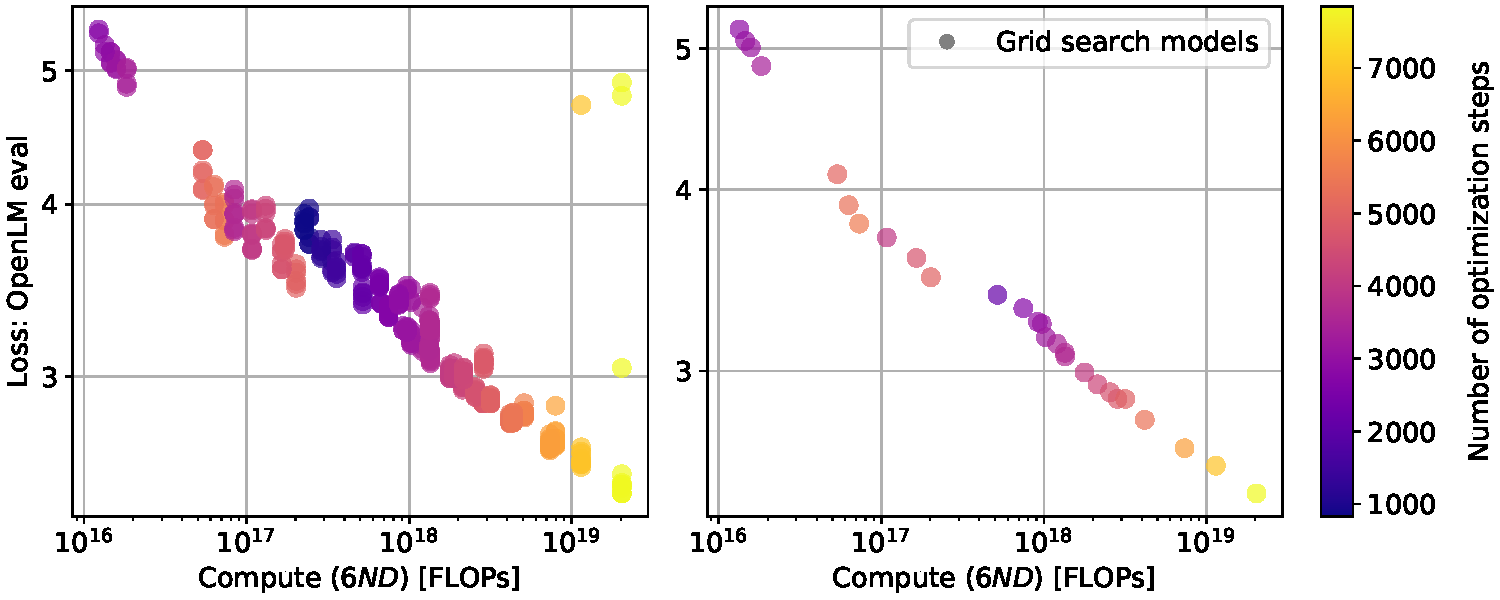
\includegraphics[width=0.98\linewidth]{figs/grid_full_color.pdf}
    \caption{\textbf{Understanding over-performing models in our grid search.}
    \emph{(left)}
    Models trained with $5.2 \times 10^{16}$ to $5.2 \times 10^{17}$ FLOPs over-perform relative to their neighbors.
    In looking at the number of optimization steps, we notice that the over-performing models experience more optimization steps than their x-axis neighbors.
    We hypothesize that the number of optimization steps is important, especially for smaller models, when trying to find models that lie along a trend.
    \emph{(right)} A view of the same phenomenon, specifically on the efficient frontier. 
    }
    \label{fig:grid_color}
\end{figure}

\paragraph{Scaling is largely predictable in-distribution (ID).}
Prior work focuses on understanding scaling using ID loss, often using training loss directly~\cite{kaplan2020scaling,chinchilla}.
Hence, we also consider Paloma~\cite{paloma} loss evaluation sets, which are designed to probe performance in specific domains.
We use Paloma's C4~\cite{c4,c4_ai2}, RedPajama~\cite{rpj}, and Falcon-RefinedWeb~\cite{refinedweb} splits to probe for ID loss.
As seen in Figure~\ref{fig:error_id}, relative error is mostly low.
Relative error is largest for the $N=1.4\text{B}, M=640$ RedPajama run at 15.4\%.
Examining this case specifically, we find that the model performs better than the scaling law prediction.
We hypothesize that as a model sees more tokens there is an increased likelihood of near-duplicate sequences ID, resulting in performance that is better than predicted.

\begin{figure}[tp]
    \centering
    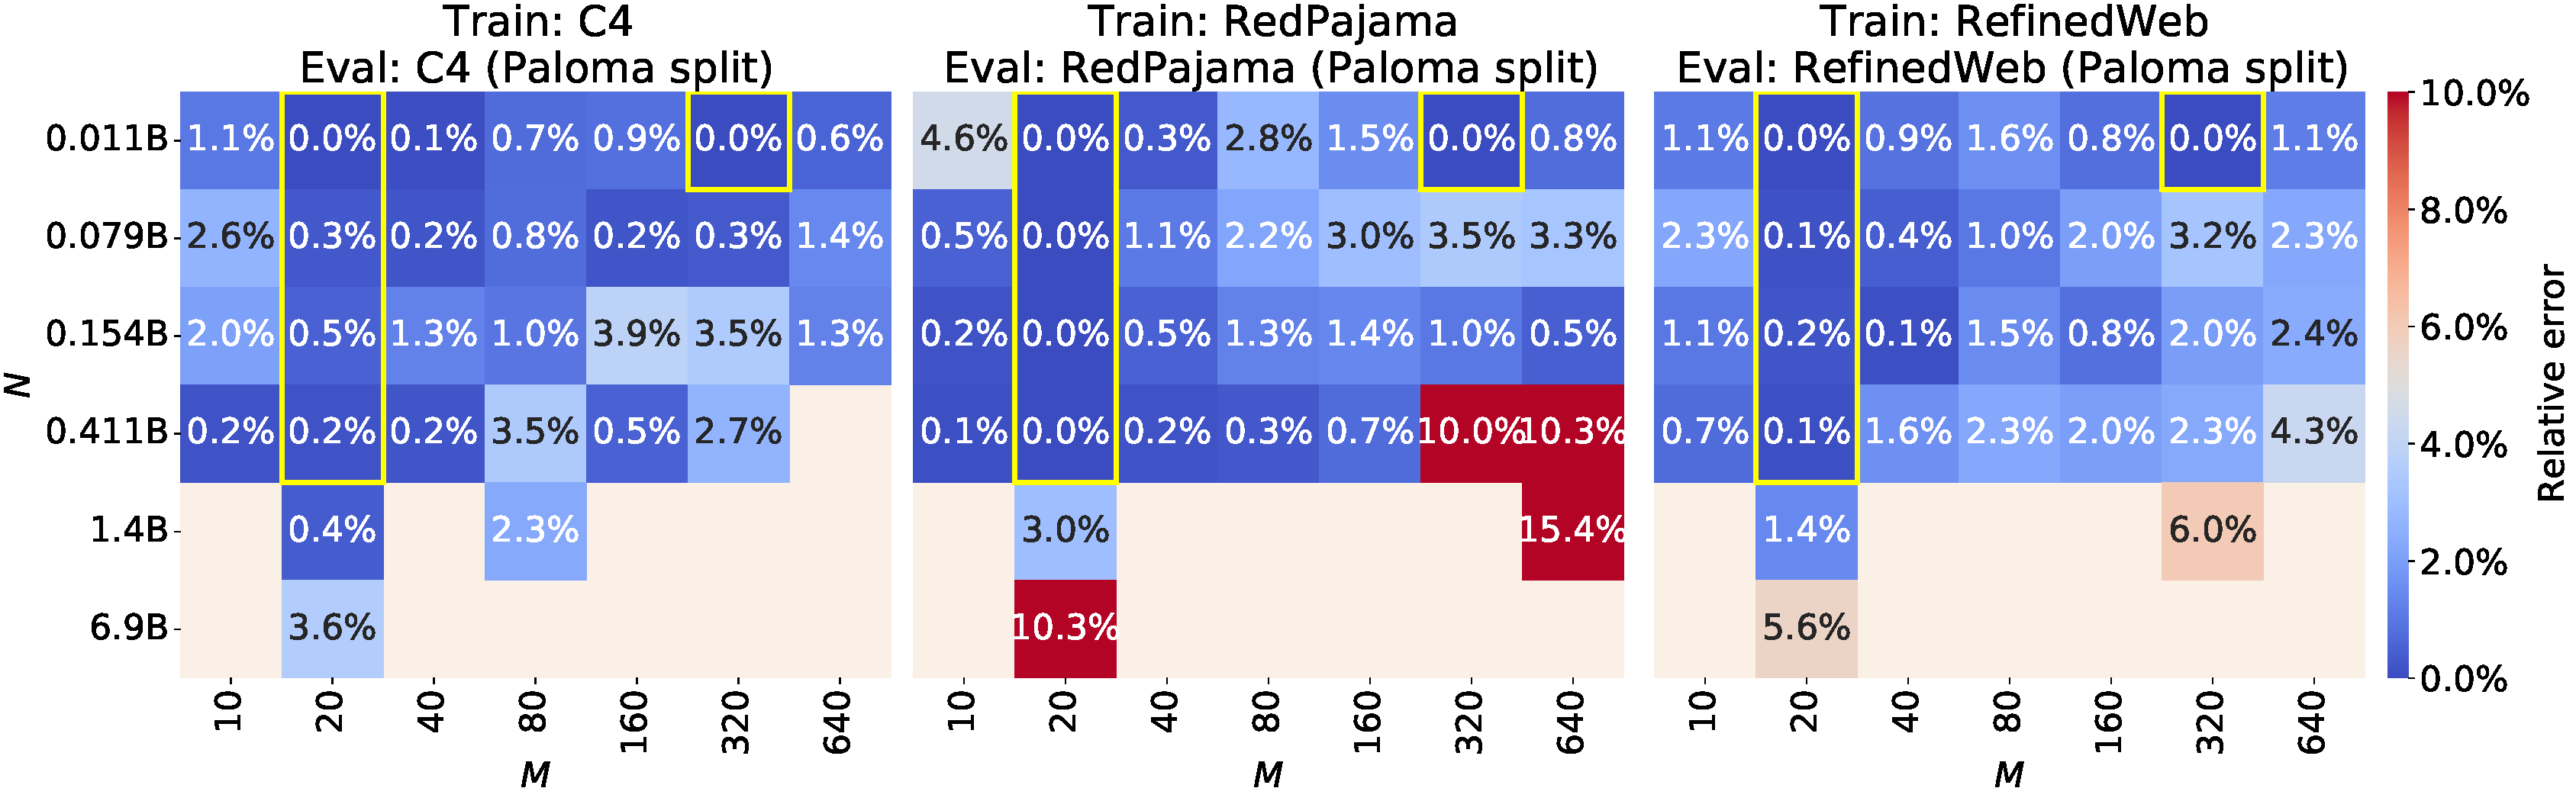
\includegraphics[width=\linewidth]{figs/error_id.pdf}
    \caption{\textbf{In-distribution (ID) settings.} Boxes highlighted in yellow correspond to data points used to fit Equation~\eqref{eq:lossCM}. Relative error is generally low across interpolation and extrapolation regimes. Relative error is largest for the RedPajama $N=1.4\text{B}, M=640$ prediction at 15.4\%. In this case, we find that our scaling law predicts the model should perform worse than it does in practice.
    }
    \label{fig:error_id}
\end{figure}

\paragraph{Relative error is stable across many choices of downstream evaluation suites.}

To understand how sensitive our investigation is to our choices of downstream evaluation sets, we consider several other options as seen in Figure~\ref{fig:eval_ablation}.
We find that our prediction errors are fairly (i) low and (ii) consistent for many choices of downstream evaluation sets including the whole suite of 46 evaluations.

\begin{figure}[tp]
    \centering
    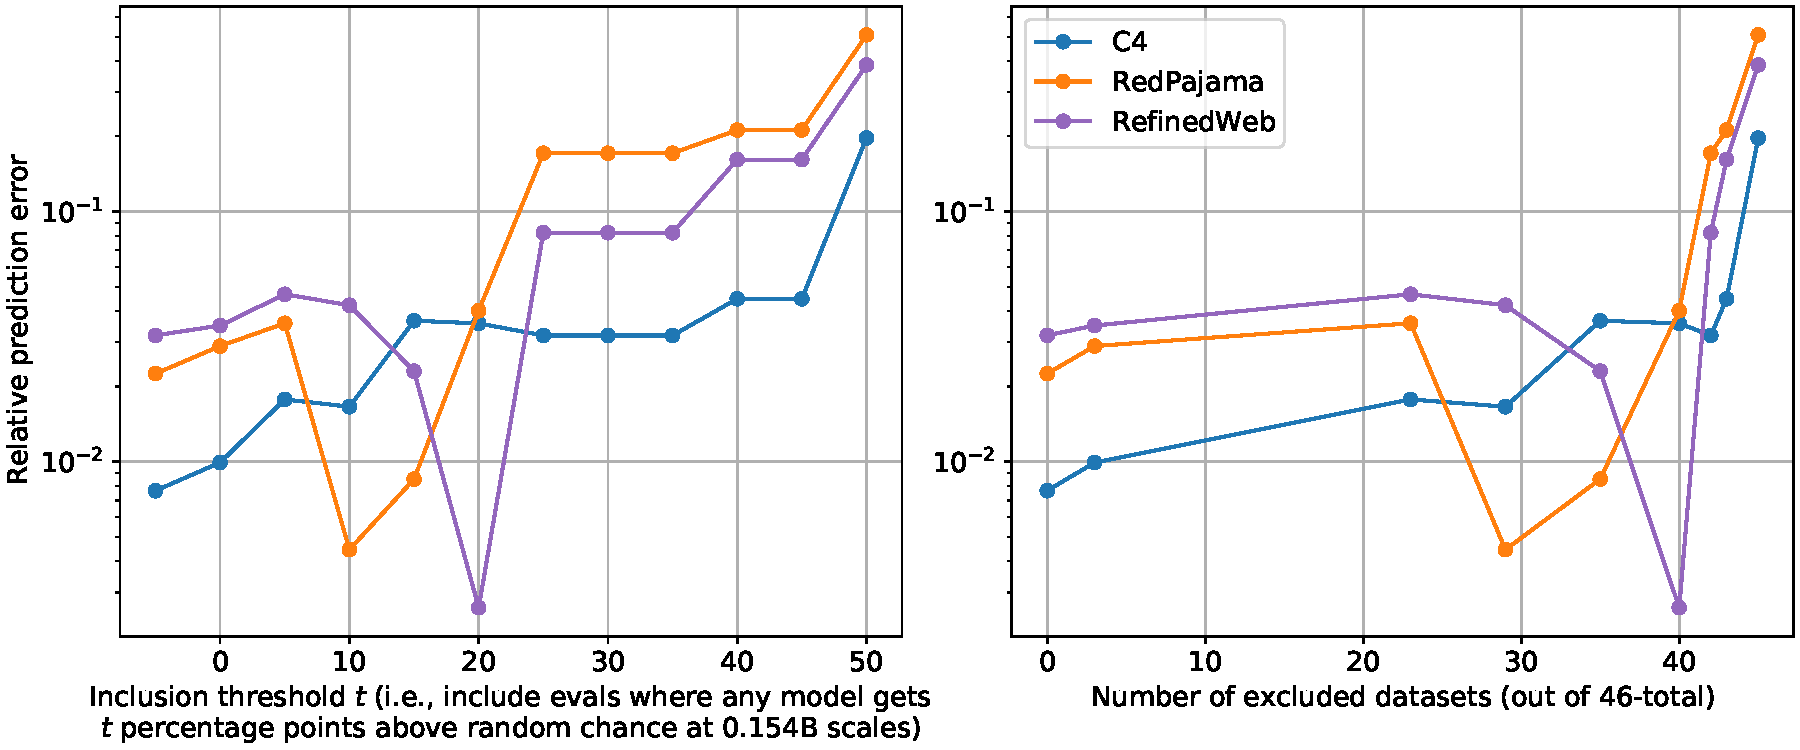
\includegraphics[width=\linewidth]{figs/eval_ablation.pdf}
    \caption{
    \textbf{Downstream evaluation set ablation for 6.9B parameter, 138B token runs.}
    Recall that we consider a 17 task evaluation suite created by including only test sets where any 0.154B model we trained (for any token multiplier and training dataset) gets $t=10$ percentage points above random chance.
    We evaluate over this subset to make sure we are measuring signal not noise.
    Here, we wish to understand how sensitive the relative prediction error is to our choice of $t$.
    \emph{(left)}
    We see that relative prediction error is fairly low before a threshold of $t=35$ (less than $10\%$ relative error).
    When too many tasks are excluded (i.e., $t\geq 40$) relative error spikes.
    Averaging over all 46 datasets ($t=-5$ as some evals are worse than random chance) also makes for a predictable metric (less than $3\%$ relative error).
    \emph{(right)}
    A parallel view, showing how many tasks are removed as $t$ increases.
    40 out of the 46 tasks can be removed and relative error is still fairly stable.
    }
    \label{fig:eval_ablation}
\end{figure}

\begin{table}[tp]
    \centering
    \footnotesize
    \caption{
    \textbf{Downstream relative prediction error at 6.9B, 138B tokens, with and without the 1.4B data point.}
    Recall in Table~\ref{tab:fit_hparams}, we introduce a $N=1.4$B, $M=20$ run to get better downstream error predictions.
    Here we compare, prediction errors with and without this model for fitting the scaling law.
    Note that without the model (i.e., rows with ``w/o 1.4B'') average top-1 predictions, over the 17 tasks. are less accurate.
    }    
    \begin{tabular}{ll|cccc|c}
        \toprule
         Scaling law fit & Train set & ARC-E & LAMBADA & OpenBook QA & HellaSwag & 17 eval  \\
          & & \cite{arc} & \cite{lambada} & \cite{OpenBookQA2018} & \cite{hellaswag} &  \\         
         \midrule
        Table~\ref{tab:fit_hparams} & C4~\cite{c4,c4_ai2} & 28.96\% &15.01\% &16.80\% &79.58\% &0.14\% \\
        Table~\ref{tab:fit_hparams} w/o 1.4B & C4~\cite{c4,c4_ai2} & 0.92\% &2.04\% &96.16\% &61.79\% &0.42\% \\\midrule
        Table~\ref{tab:fit_hparams} & RedPajama~\cite{rpj} & 5.21\% &14.39\% &8.44\% &25.73\% &0.05\% \\
        Table~\ref{tab:fit_hparams} w/o 1.4B & RedPajama~\cite{rpj} & 8.13\% &11.07\% &7.56\% &30.98\% &10.64\% \\\midrule
        Table~\ref{tab:fit_hparams} & RefinedWeb~\cite{refinedweb} & 26.06\% &16.55\% &1.92\% &81.96\% &2.94\% \\
        Table~\ref{tab:fit_hparams} w/o 1.4B & RefinedWeb~\cite{refinedweb} & 15.39\% &6.26\% &6.79\% &6.52\% &15.79\% \\
        \midrule
    \end{tabular}
    \label{tab:downstream_wo}
\end{table}

\paragraph{Scaling can break down when under-training.}

\begin{figure}[tp]
    \centering
    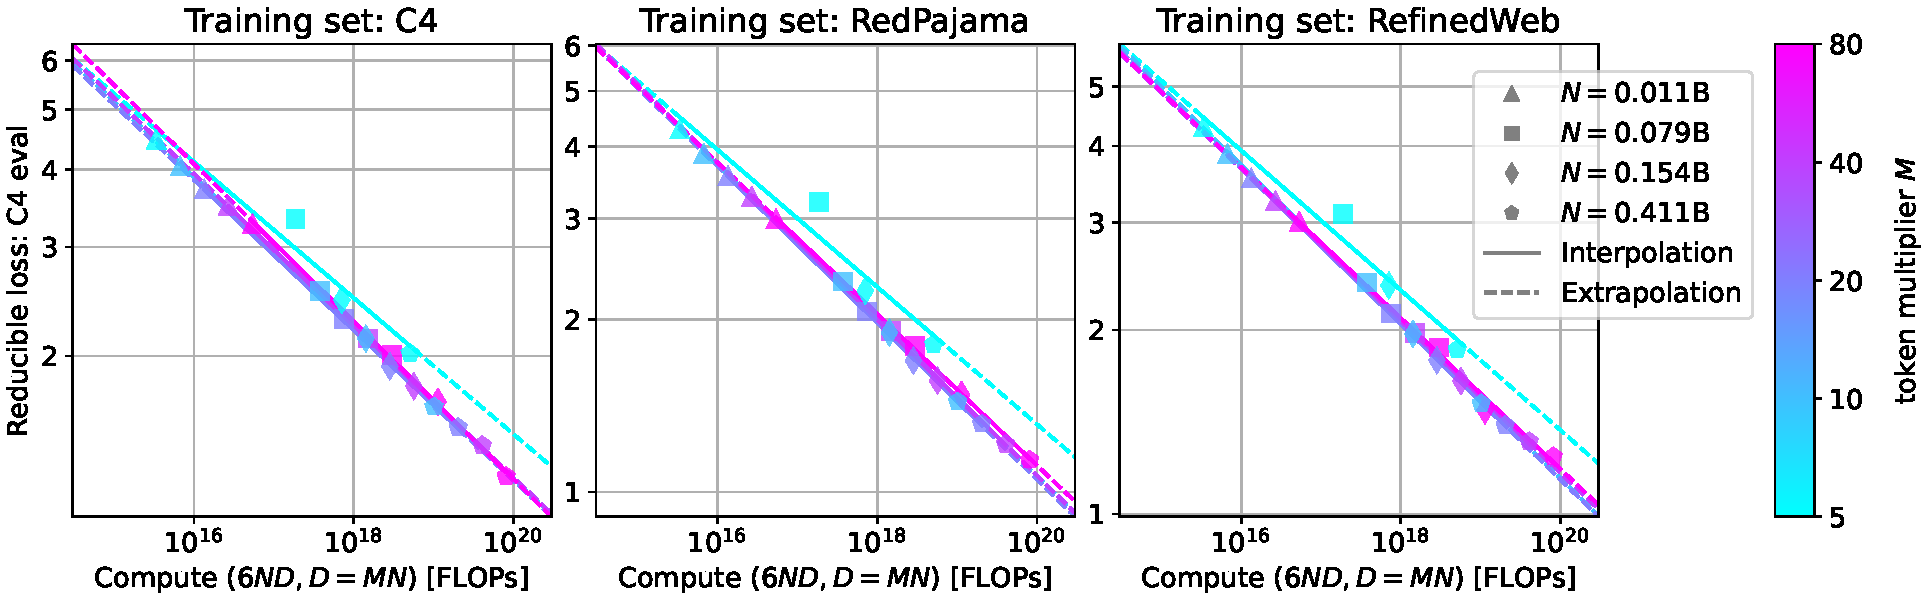
\includegraphics[width=\linewidth]{figs/emperical_small.pdf}
    \caption{\textbf{Scaling with small token multipliers.} For smaller multipliers (e.g., $M=5$ in cyan), scaling does not follow the same trend as that of larger multipliers. Additionally, many token multipliers (e.g., $M \in \{10, 20, 40, 80\}$) garner points close to the compute-optimal frontier.}
    \label{fig:emperical_small}
\end{figure}

We find that when a token multiple is too small (i.e., under-training regime), scaling appears unreliable.
In Figure~\ref{fig:emperical_small} we see for $M=5$ the scaling trend is different.
We hypothesize that tuning hyperparameters (e.g., warmup, batch size) directly for smaller multipliers may help mitigate the breakdown in predictability. 

\paragraph{Scaling can be unpredictable out-of-distribution (OOD).}

Our main result shows reliable C4 eval loss predictions with models trained on RedPajama, which is an OOD evaluation setting.
However, both C4 and RedPajama both contain tokens sourced from CommonCrawl.

To further probe OOD performance, we measure the relative error of scaling laws fit to models trained on C4 and evaluated on Paloma's 100 programming languages~\cite{paloma}, Paloma's Penn Tree Bank (PTB) split~\cite{ptb}, and a German version of C4~\cite{c4_ai2}.
Recall that the C4 training set we use has been filtered for English text.
Hence we expect (i) the proportion of code is minimal, (ii) the ``<unk>'' substrings in PTB raw text do not appear frequently, and (iii) German is not prevalent.
We notice that extrapolation relative error tends to be high for large $M, N$ on programming languages and PTB (Figure~\ref{fig:error_ood} \emph{(left, center)}).
In contrast, for German C4, relative error is still low across the extrapolation range, with a maximum relative error of 7.6\% at the $N=$1.4B, $M=80$ scale (Figure~\ref{fig:error_ood} \emph{(right)}). 
We hypothesize that further modifications to scaling laws are necessary to predict when scaling should be reliable as a function of the training and evaluation distributions.

\begin{figure}[tp]
    \centering
    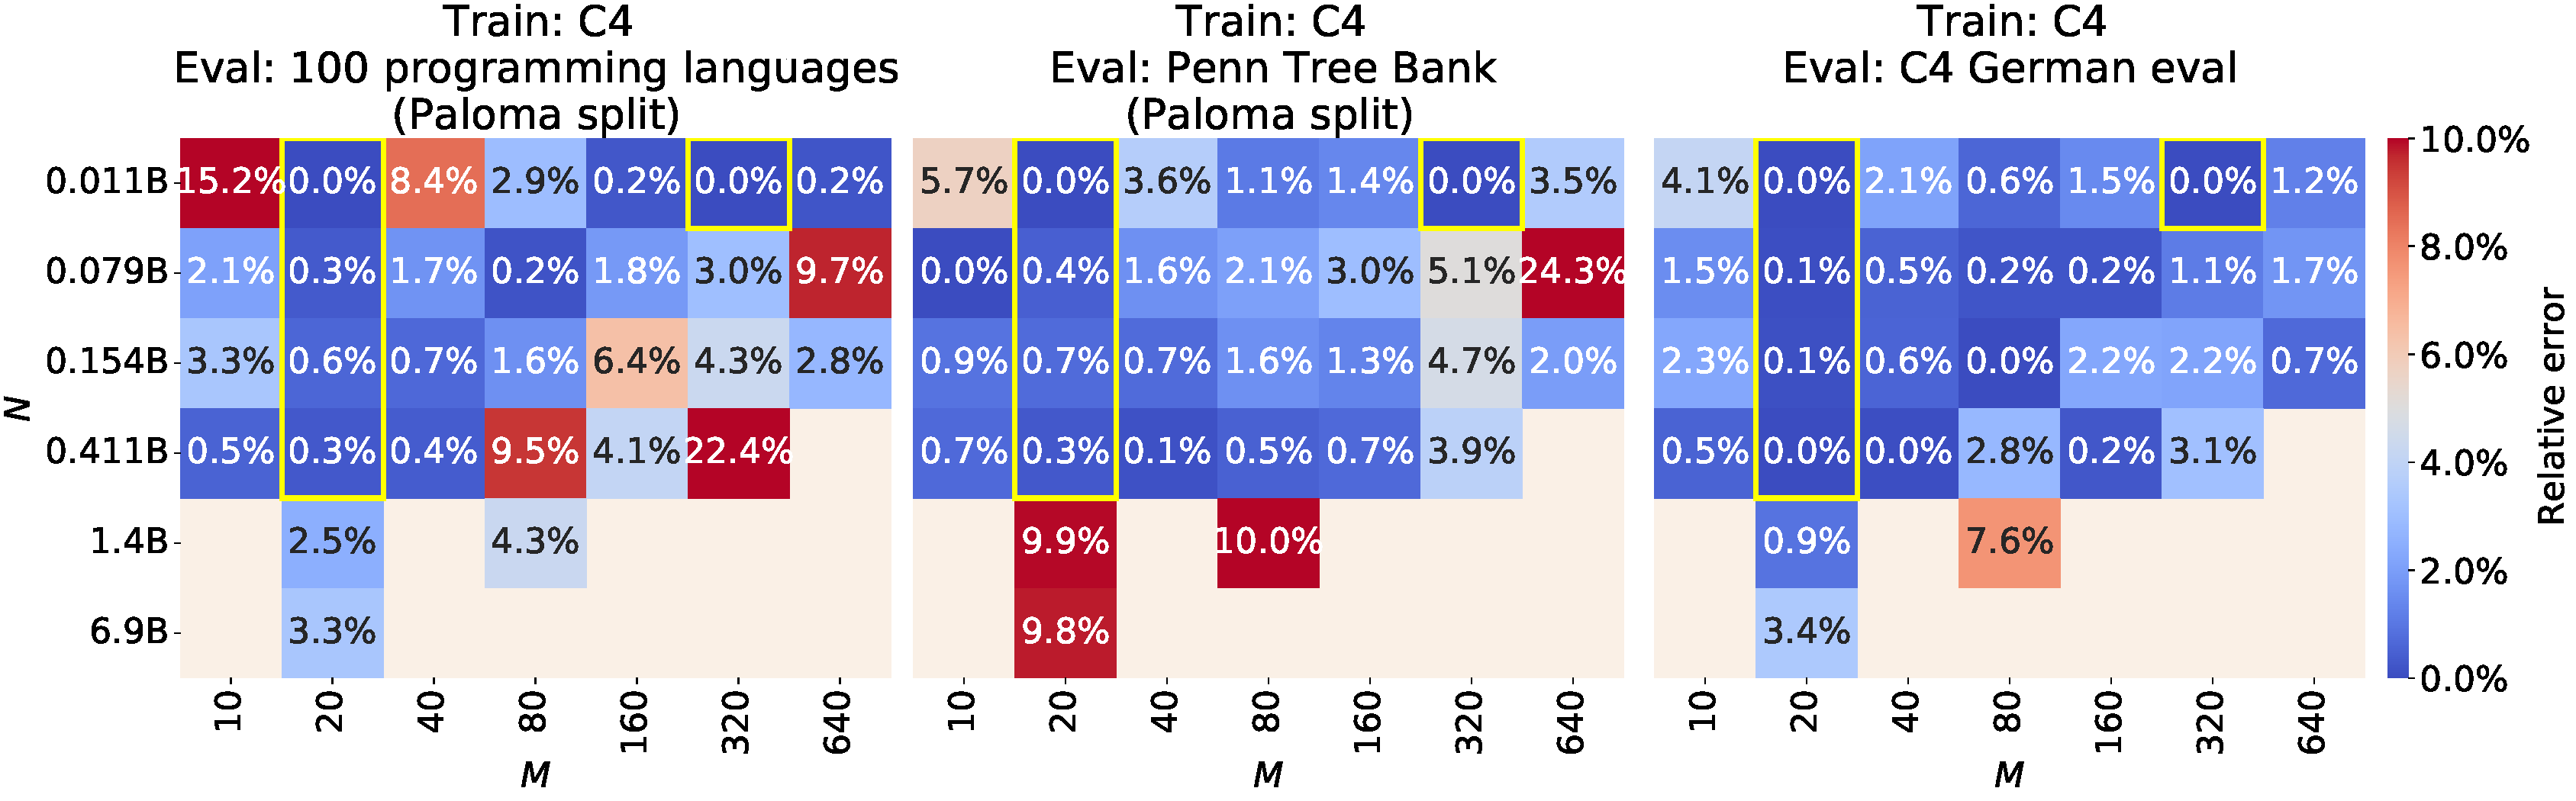
\includegraphics[width=\linewidth]{figs/error_ood.pdf}
    \caption{\textbf{Out-of-distribution (OOD) settings.} Boxes highlighted in yellow correspond to data points used to fit Equation~\eqref{eq:lossCM}.
    Recall that the C4 training set is English-filtered. Relative error can spike, suggesting unreliable scaling, for \emph{(left)} programming languages and \emph{(center)} Penn Tree Bank, which contains many frequently occurring, uncommon substrings.
    However, scaling is relatively reliable when evaluating on \emph{(right)} German.
    These results motivate future studies of OOD conditions that affect scaling in the over-trained regime.
    }
    \label{fig:error_ood}
\end{figure}


\paragraph{Small-scale experiments can predict average downstream top-1 error.}
\begin{figure}[tp]
    \centering
    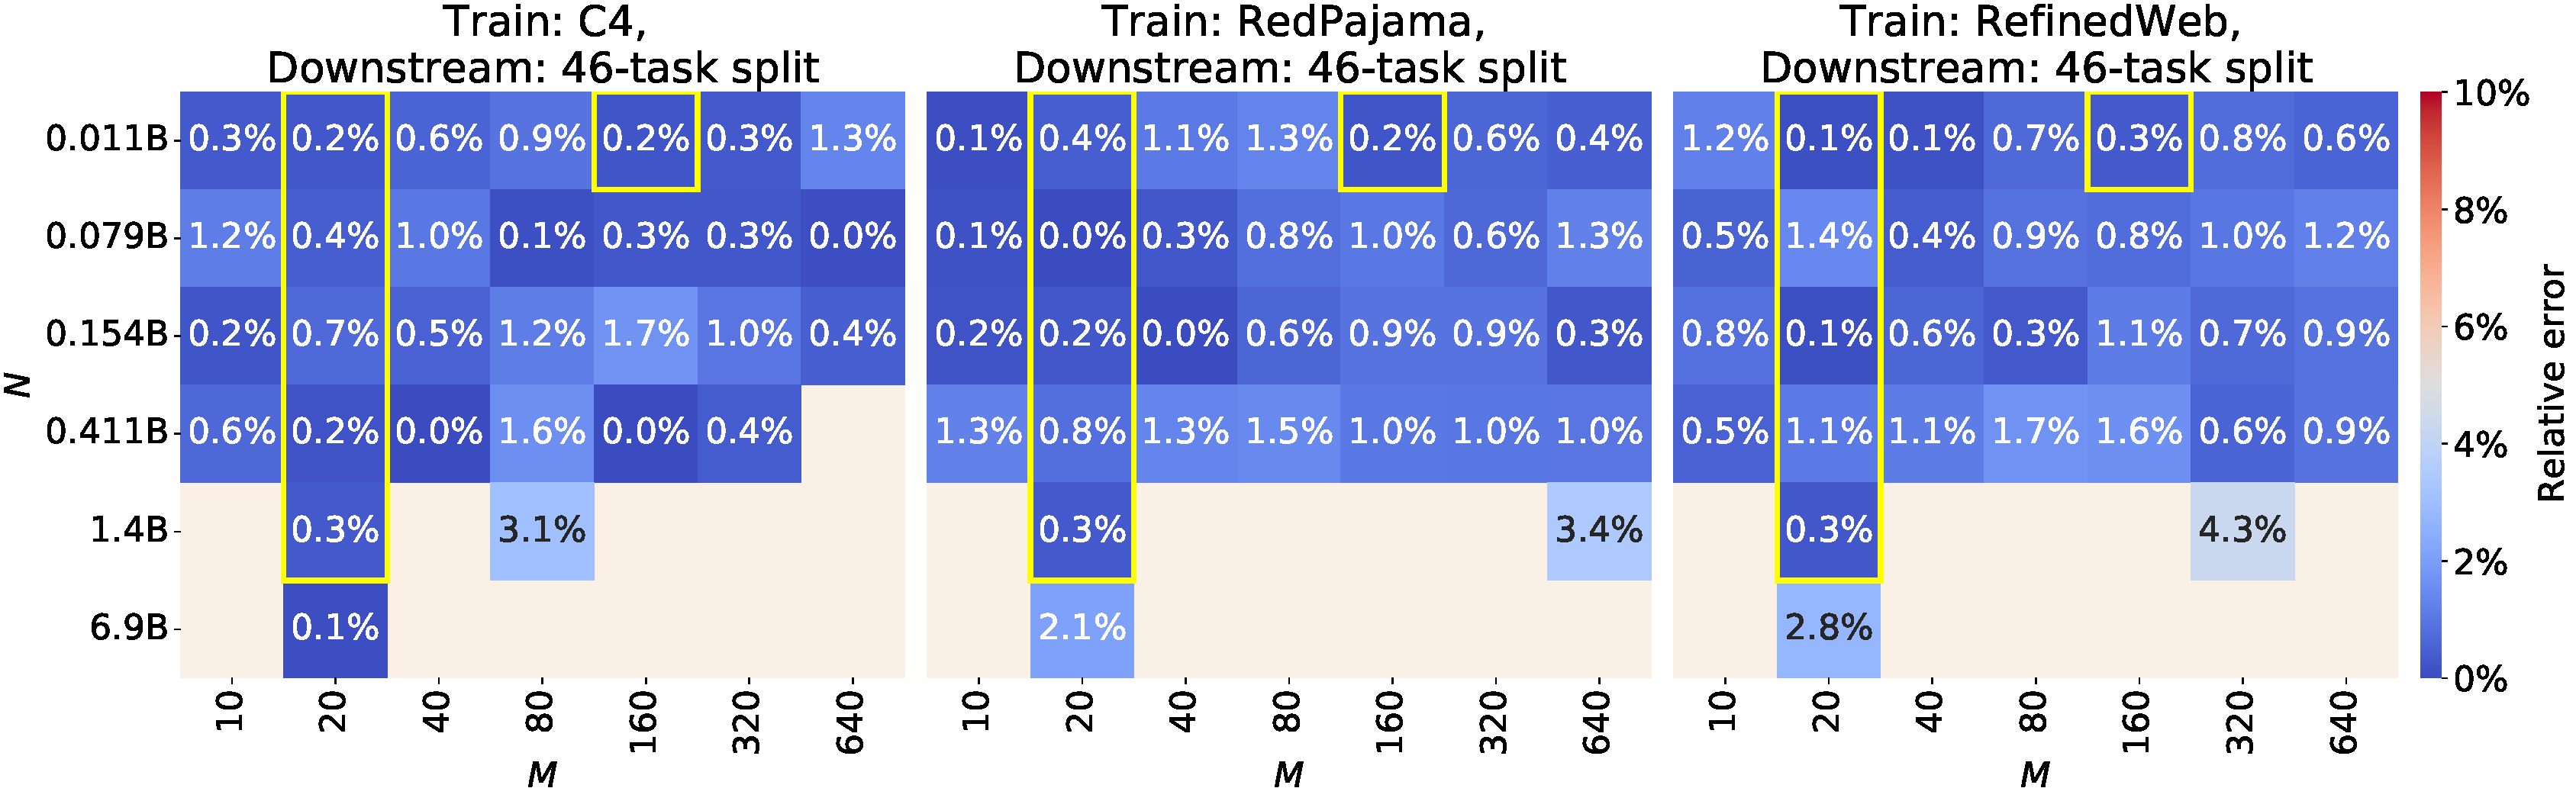
\includegraphics[width=\linewidth]{figs/error_downstream_all.pdf}
    \caption{\textbf{Relative error on average top-1 predictions (46 task split).}
    Boxes highlighted in yellow correspond to data points used to fit Equation~\eqref{eq:errL}.
    Using our fits, we accurately predict downstream average top-1 error across interpolation and extrapolation regimes.
    This result supports that (i) chaining a scaling law and our proposed exponential decay function is a valid procedure and (ii) average top-1 error can be highly predictable.
    }
    \label{fig:error_downstream_all}
\end{figure}
To verify that chaining Equations~\eqref{eq:lossCM} and \eqref{eq:errL} is effective in practice, we collect C4 eval loss and downstream error pairs for the configurations in Table~\ref{tab:fit_hparams}.
In Figure~\ref{fig:error_downstream_all}, we look at relative error for our scaling predictions in the context of Average top-1 error over 46 evals and in Figure~\ref{fig:error_downstream_subset} over the high-signal 17 eval subset.
We again notice reliable scaling in interpolation and extrapolation regimes, suggesting the validity of our procedure to predict downstream average top-1 error.


\begin{figure}[tp]
    \centering
    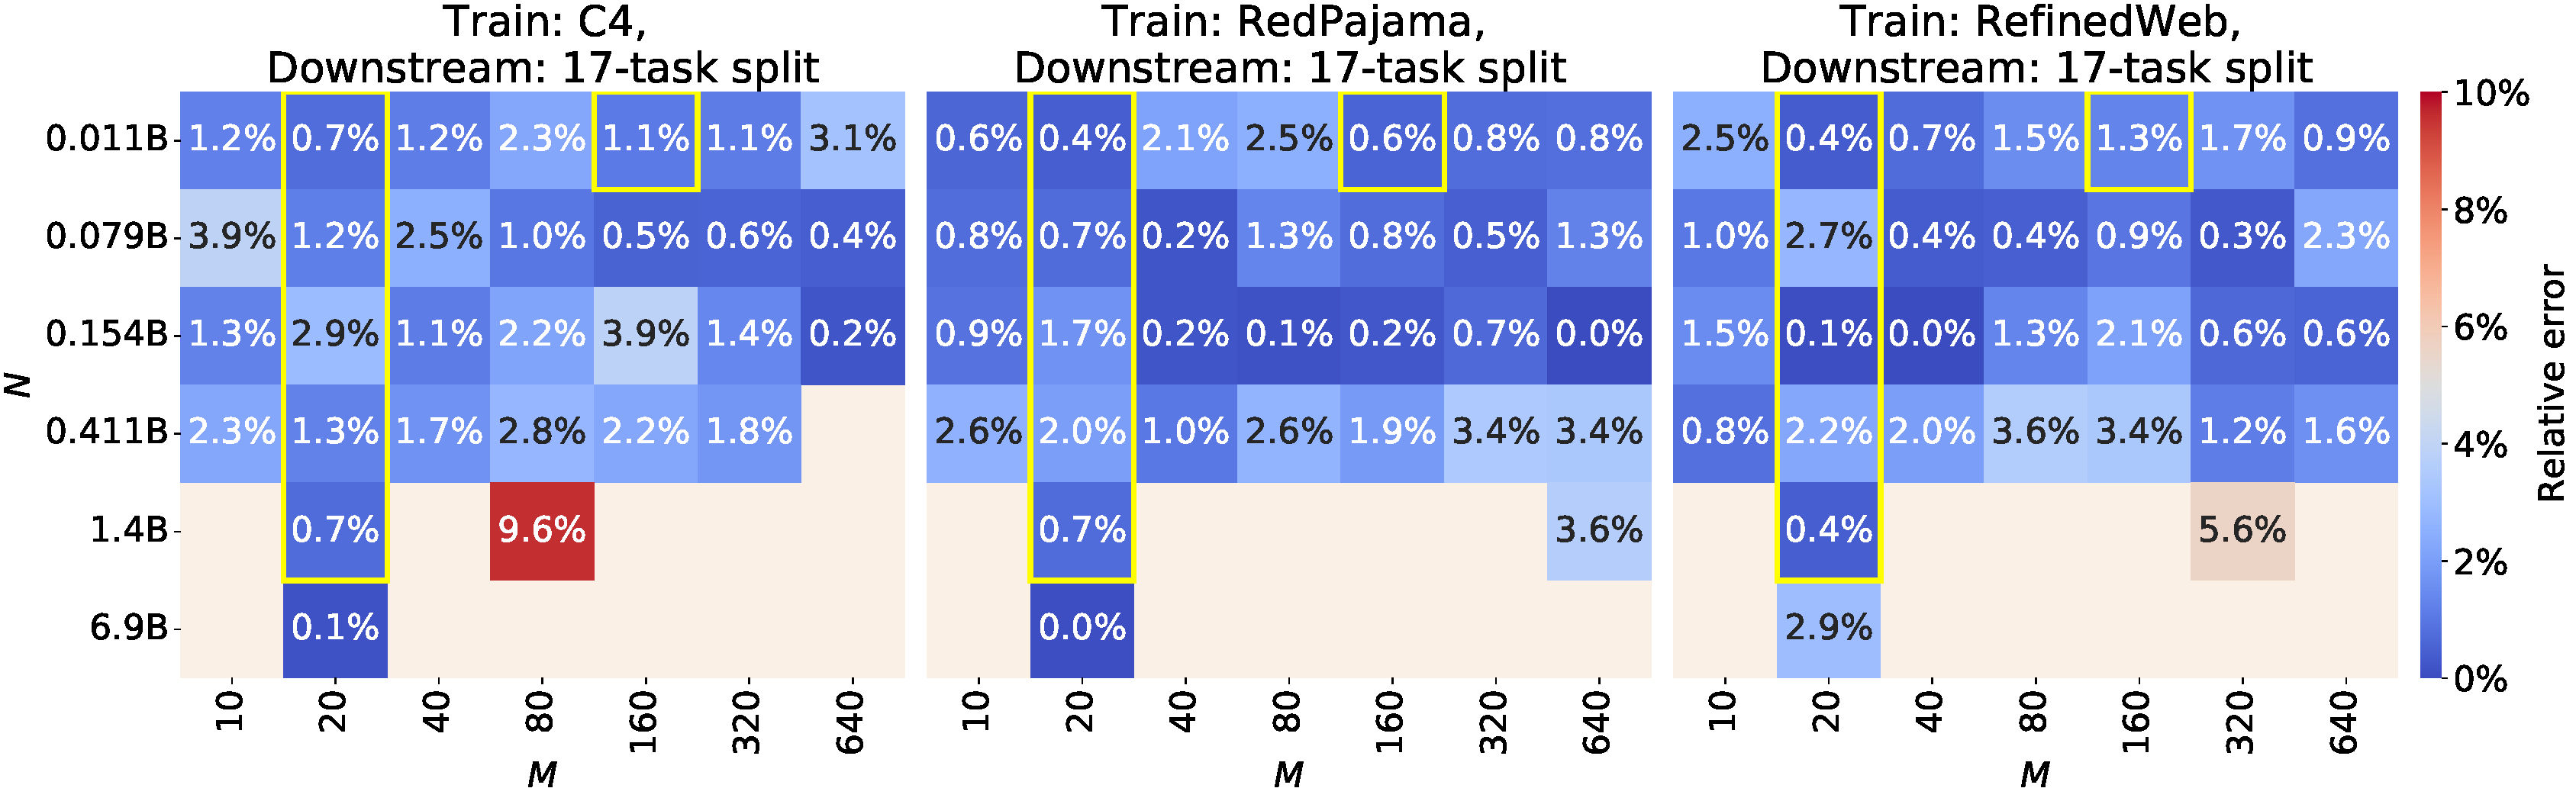
\includegraphics[width=\linewidth]{figs/error_downstream_subset.pdf}
    \caption{\textbf{Relative error on average top-1 predictions (17 task split).}
    Boxes highlighted in yellow correspond to data points used to fit Equation~\eqref{eq:errL}.
    Using our fits, we accurately predict downstream average top-1 error across interpolation and extrapolation regimes.
    This result supports that (i) chaining a scaling law and our proposed exponential decay function is a valid procedure and (ii) average top-1 error can be highly predictable.
    }
    \label{fig:error_downstream_subset}
\end{figure}

\paragraph{Loss evaluation ablations for downstream trends.}
Figure~\ref{fig:downstream_corr_ablation} presents the correlation between downstream error and loss evaluated on different validation sets (C4, RedPajama, and RefinedWeb). Regardless of the validation set (x-axis), models follow the exponential decay relationship given in Equation~\eqref{eq:errL}, suggesting the choice of validation loss is not critical for the appearance of this phenomenon.

\begin{figure}[tp]
    \centering
    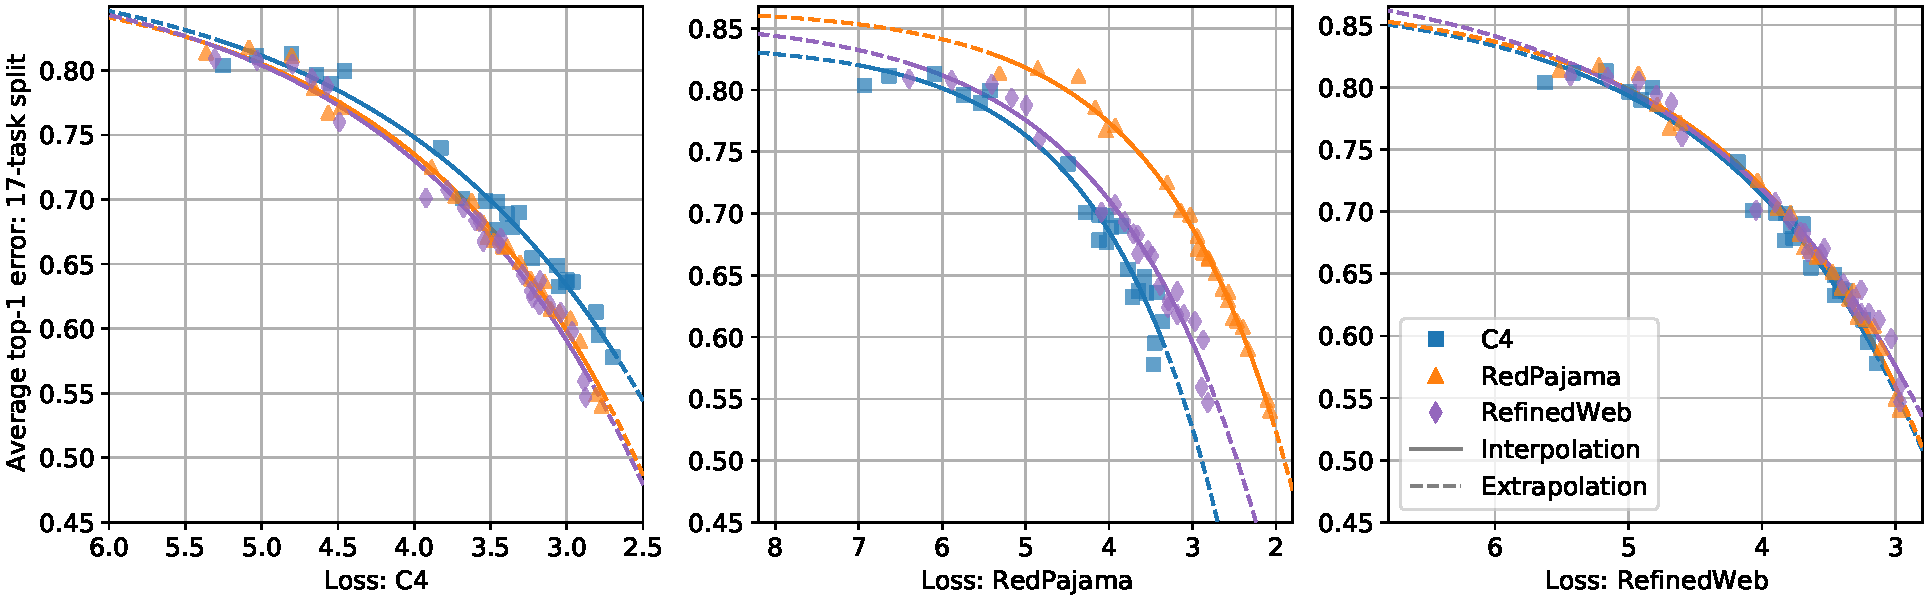
\includegraphics[width=0.98\linewidth]{figs/downstream_corr_ablation.pdf}
    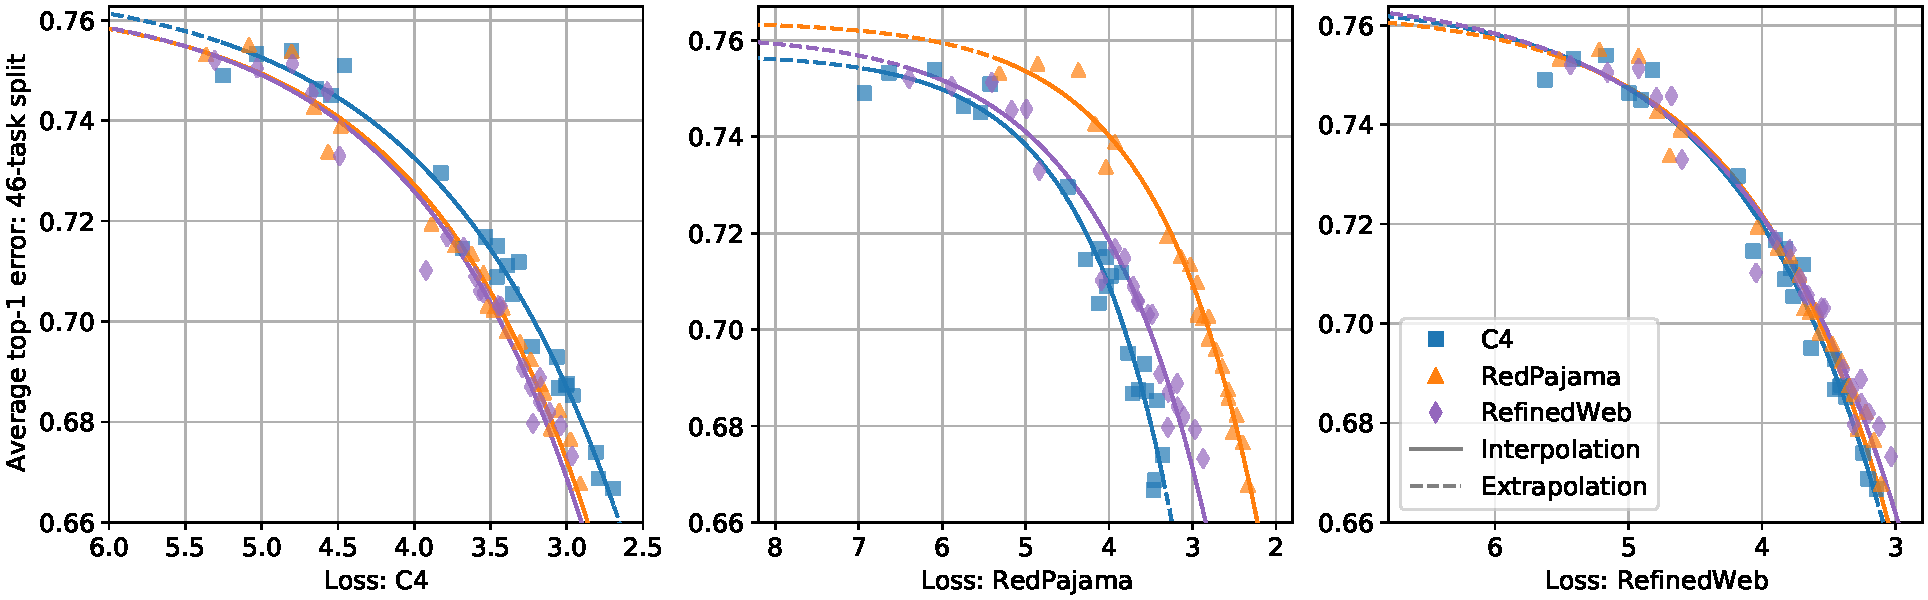
\includegraphics[width=0.98\linewidth]{figs/downstream_corr_ablation_all.pdf}
    \caption{\textbf{Correlation between average top-1 error and evaluation loss.}
    We observe that regardless of evaluation loss distribution (x-axis), models tend to follow Equation~\eqref{eq:errL}.
    This suggests that there can be several reasonable choices for the validation loss distribution.
    Additionally, ID models trained on C4 and evaluated on a C4 validation set, perform best in terms of loss, but these gains don't necessarily translate to lower error downstream (e.g., \emph{(left column)}).
    This suggests \emph{the need to fit Equation~\eqref{eq:errL} per dataset} and also suggests comparing models trained on different data distributions with a single loss evaluation can be misleading.
    }
    \label{fig:downstream_corr_ablation}
\end{figure}

\paragraph{Investing more compute in a scaling law makes it more predictive.}

\begin{figure}[t!]
    \centering
    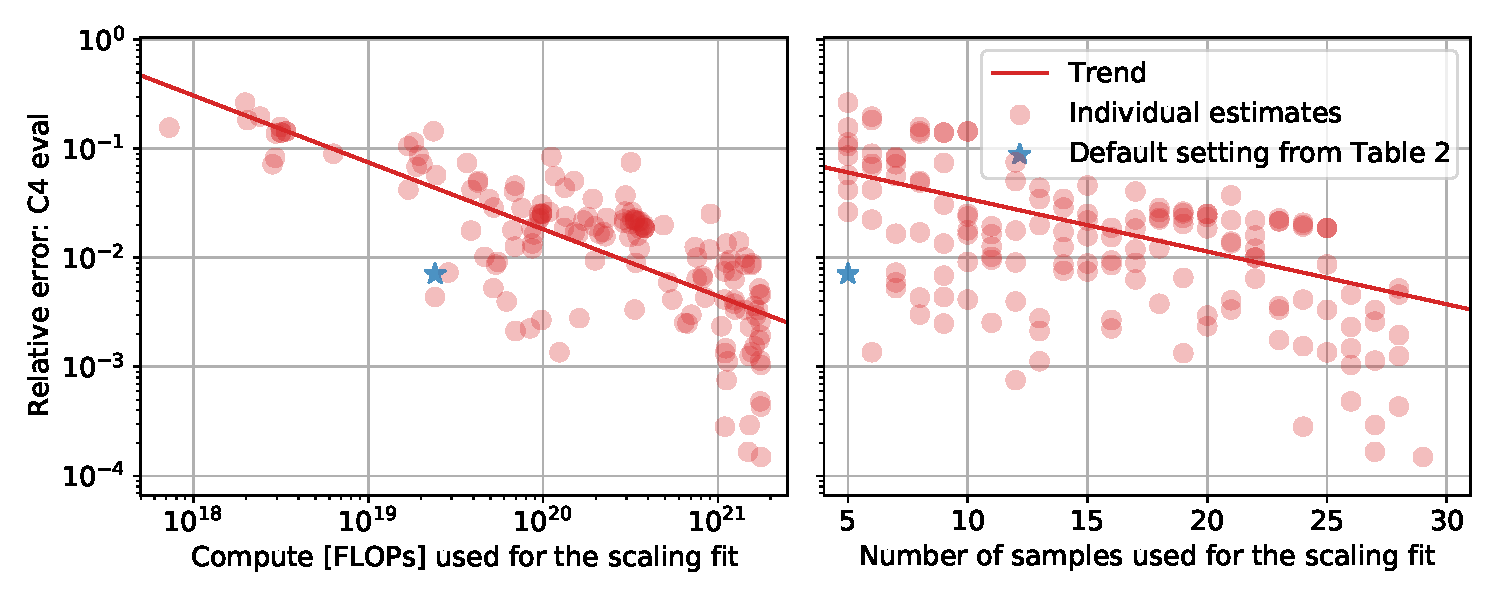
\includegraphics[width=0.98\linewidth]{figs/error_vs.pdf}
    \caption{\textbf{Trade-offs between scaling law for loss fitting considerations and reliability.} Each red circle represents a scaling law fit to Equation~\eqref{eq:lossCM} with as many as 29 models trained on RedPajama. Specifically, a grid formed by $N \in \{0.011\text{B}, 0.079\text{B}, 0.154\text{B}, 0.411\text{B}\}, M \in \{5, 10, 20, 40, 80, 160, 320\}$ gives 28 models and a $N=1.4B, M=20$ run gives the last model.
    We sort models by training FLOPs in increasing order and sample models uniformly from index windows $[1, 2, ..., n]$ for $n \in [5, 6, .., 29]$ to fit Equation~\eqref{eq:lossCM}.
    The blue star represents the default configuration presented in Table~\ref{tab:fit_hparams}. The prediction target is a $N=1.4B, M=640\text{ }(D=900\text{B})$ model. As the amount of compute \emph{(left)} and the number of points \emph{(right)} used to fit the scaling law increases, relative error trends downwards. Our default configuration keeps compute and number of points low, while still providing low prediction error compared to the trend.}
    \label{fig:error_vs}
\end{figure}

\begin{figure}
    \centering
    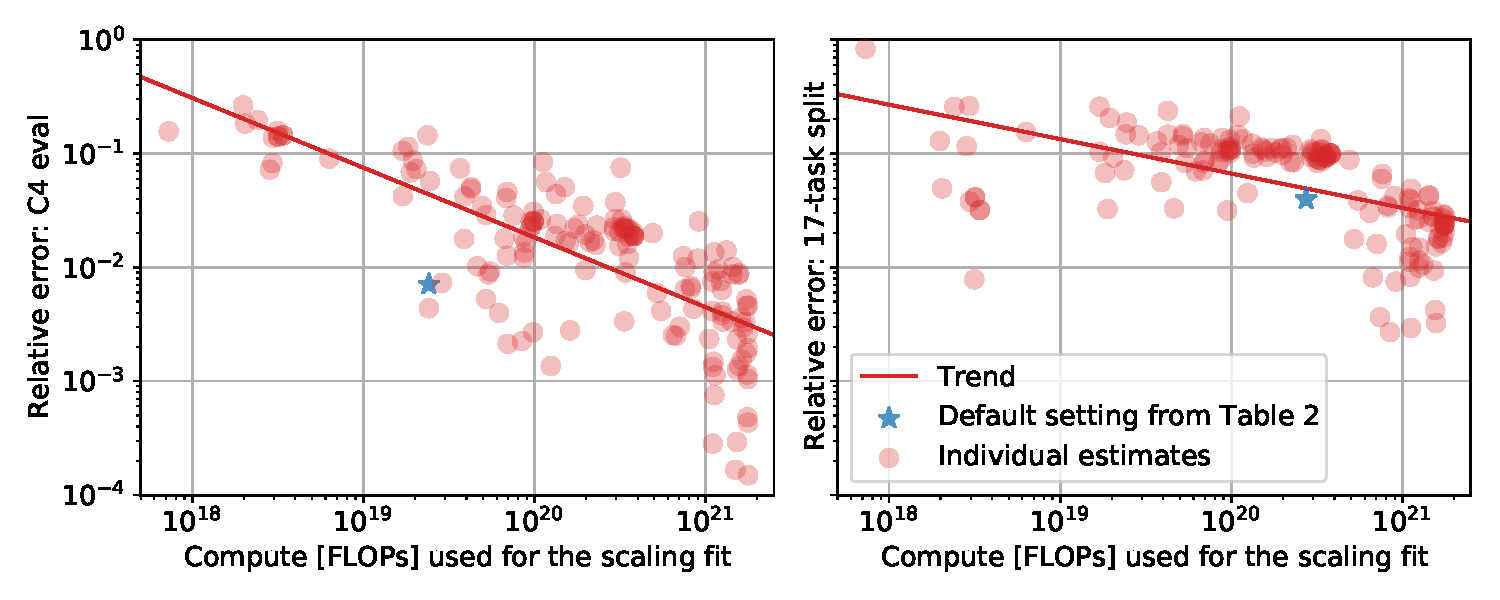
\includegraphics[width=0.98\linewidth]{figs/error_vs_1b.pdf}
    \caption{
    \textbf{Compute vs. relative error for the 1.4B, 900B token RedPajama run.}
    \emph{(left)} The compute necessary to accurately predict loss is less than that needed to accurately predict \emph{(right)} average downstream error.
    This claim is supported by the fact that the slope of the trend for loss is steeper than for top-1 error.
    These findings corroborate Figure~\ref{fig:error_vs_7b}.
    }
    \label{fig:error_vs_1b}
\end{figure}

\begin{figure}
    \centering
    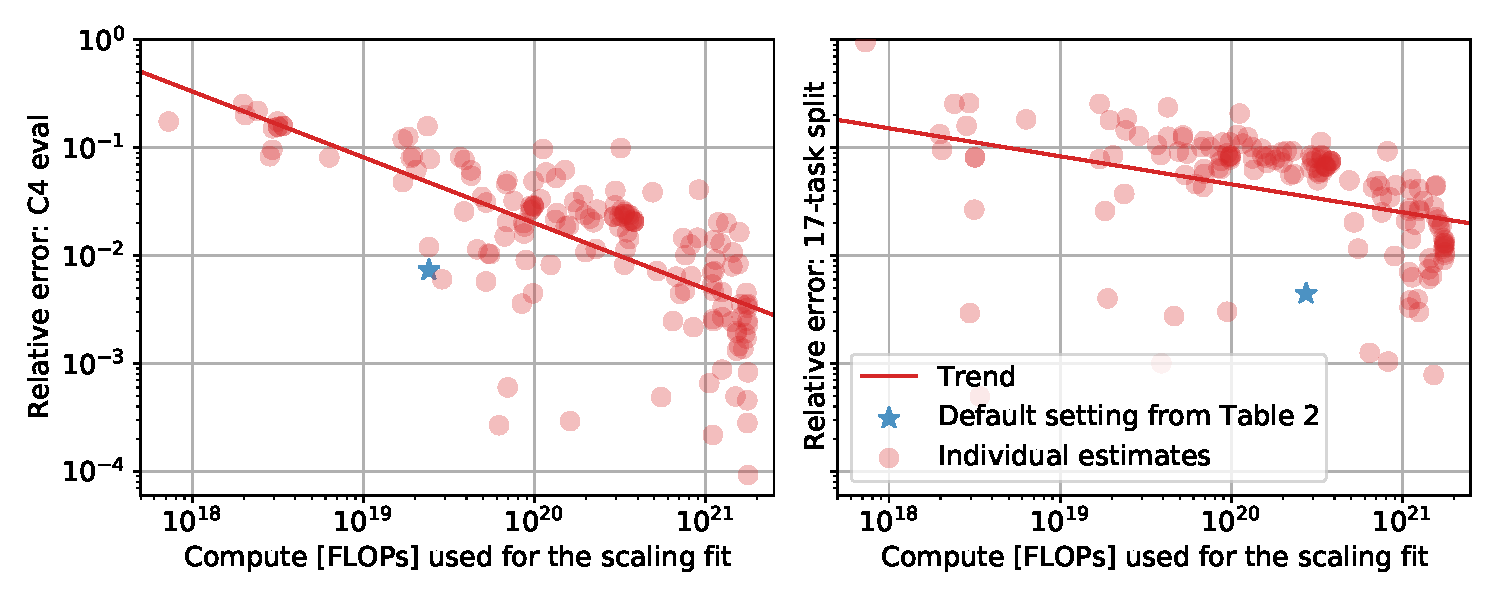
\includegraphics[width=0.98\linewidth]{figs/error_vs_7b.pdf}
    \caption{
    \textbf{Compute vs. relative error for the 6.9B, 138B token RedPajama run.}
    \emph{(left)} The compute necessary to accurately predict loss is less than that needed to accurately predict \emph{(right)} average downstream error.
    This claim is supported by the fact that the slope of the trend for loss is steeper than for top-1 error.
    These findings corroborate Figure~\ref{fig:error_vs_1b}.
    }
    \label{fig:error_vs_7b}
\end{figure}

Thus far we have looked at standard configurations from Table~\ref{tab:fit_hparams} to construct our scaling laws, mainly to demonstrate extrapolation to larger $N, M$.
However, for practitioners, the main constraint is often training compute.
Hence, we wish to understand the trade-offs between the amount of compute invested in creating a scaling law and the relative error of the resulting law in the over-trained regime.
In Figure~\ref{fig:error_vs}~\emph{(left)}, we see that as one increases the amount of compute, it is possible to get better fits with lower relative error.
In Figure~\ref{fig:error_vs}~\emph{(right)}, we see a similar trend as one increases the number of data points used to fit a scaling law.
Blue stars indicate the configurations from Table~\ref{tab:fit_hparams}, which provide accurate predictions relative to the general trends---hinting at their usefulness for our investigation.
In Figures~\ref{fig:error_vs_1b} and~\ref{fig:error_vs_7b} we repeat the compute analysis comparing trade-offs for loss prediction and error prediction for our RedPajama 1.4B parameter, 900B token and 6.9B parameter, 138B token runs respectively.
We find that less compute is generally necessary to construct a loss scaling law that achieves the same relative error as that of an error prediction scaling law.

\begin{figure}[tp]
    \centering
    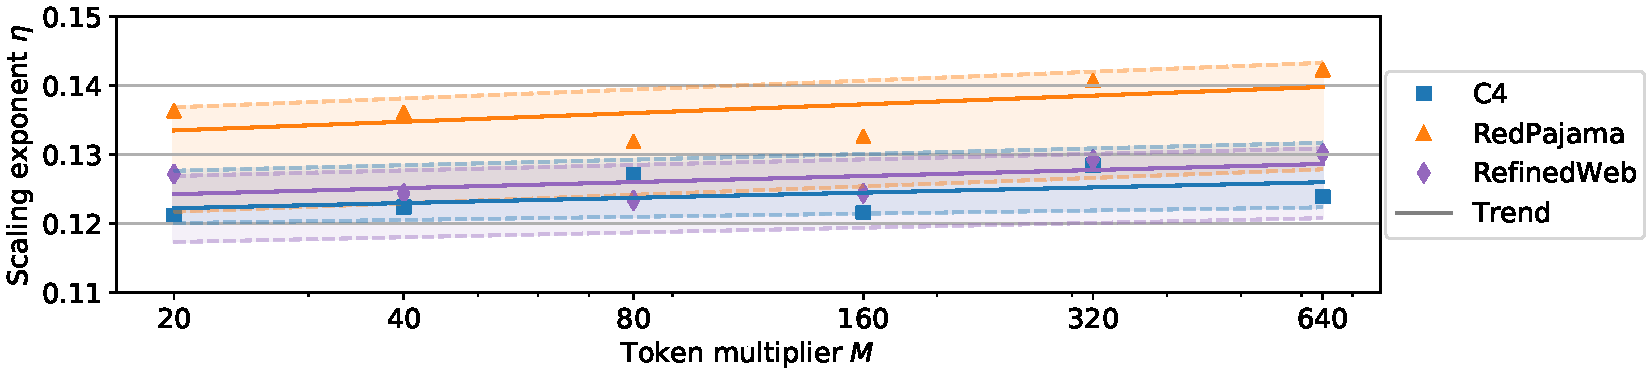
\includegraphics[width=\linewidth]{figs/slopes.pdf}
    \caption{
    \textbf{Scaling exponent vs. token multiplier.} 
    In Figure~\ref{fig:emperical}, we notice roughly parallel lines (i.e., roughly constant scaling exponent $\eta$) in the $\log$-$\log$ plot of loss vs. compute, even as the token multiplier $M$ changes.
    Here we plot $\eta$ vs. $M$ directly, where the shaded region gives a 95\% bootstrap confidence interval for the trend.
    This view supports that $\eta$ is relatively constant.
    }
    \label{fig:slopes}
\end{figure}

\begin{figure}[tp]
    \centering
    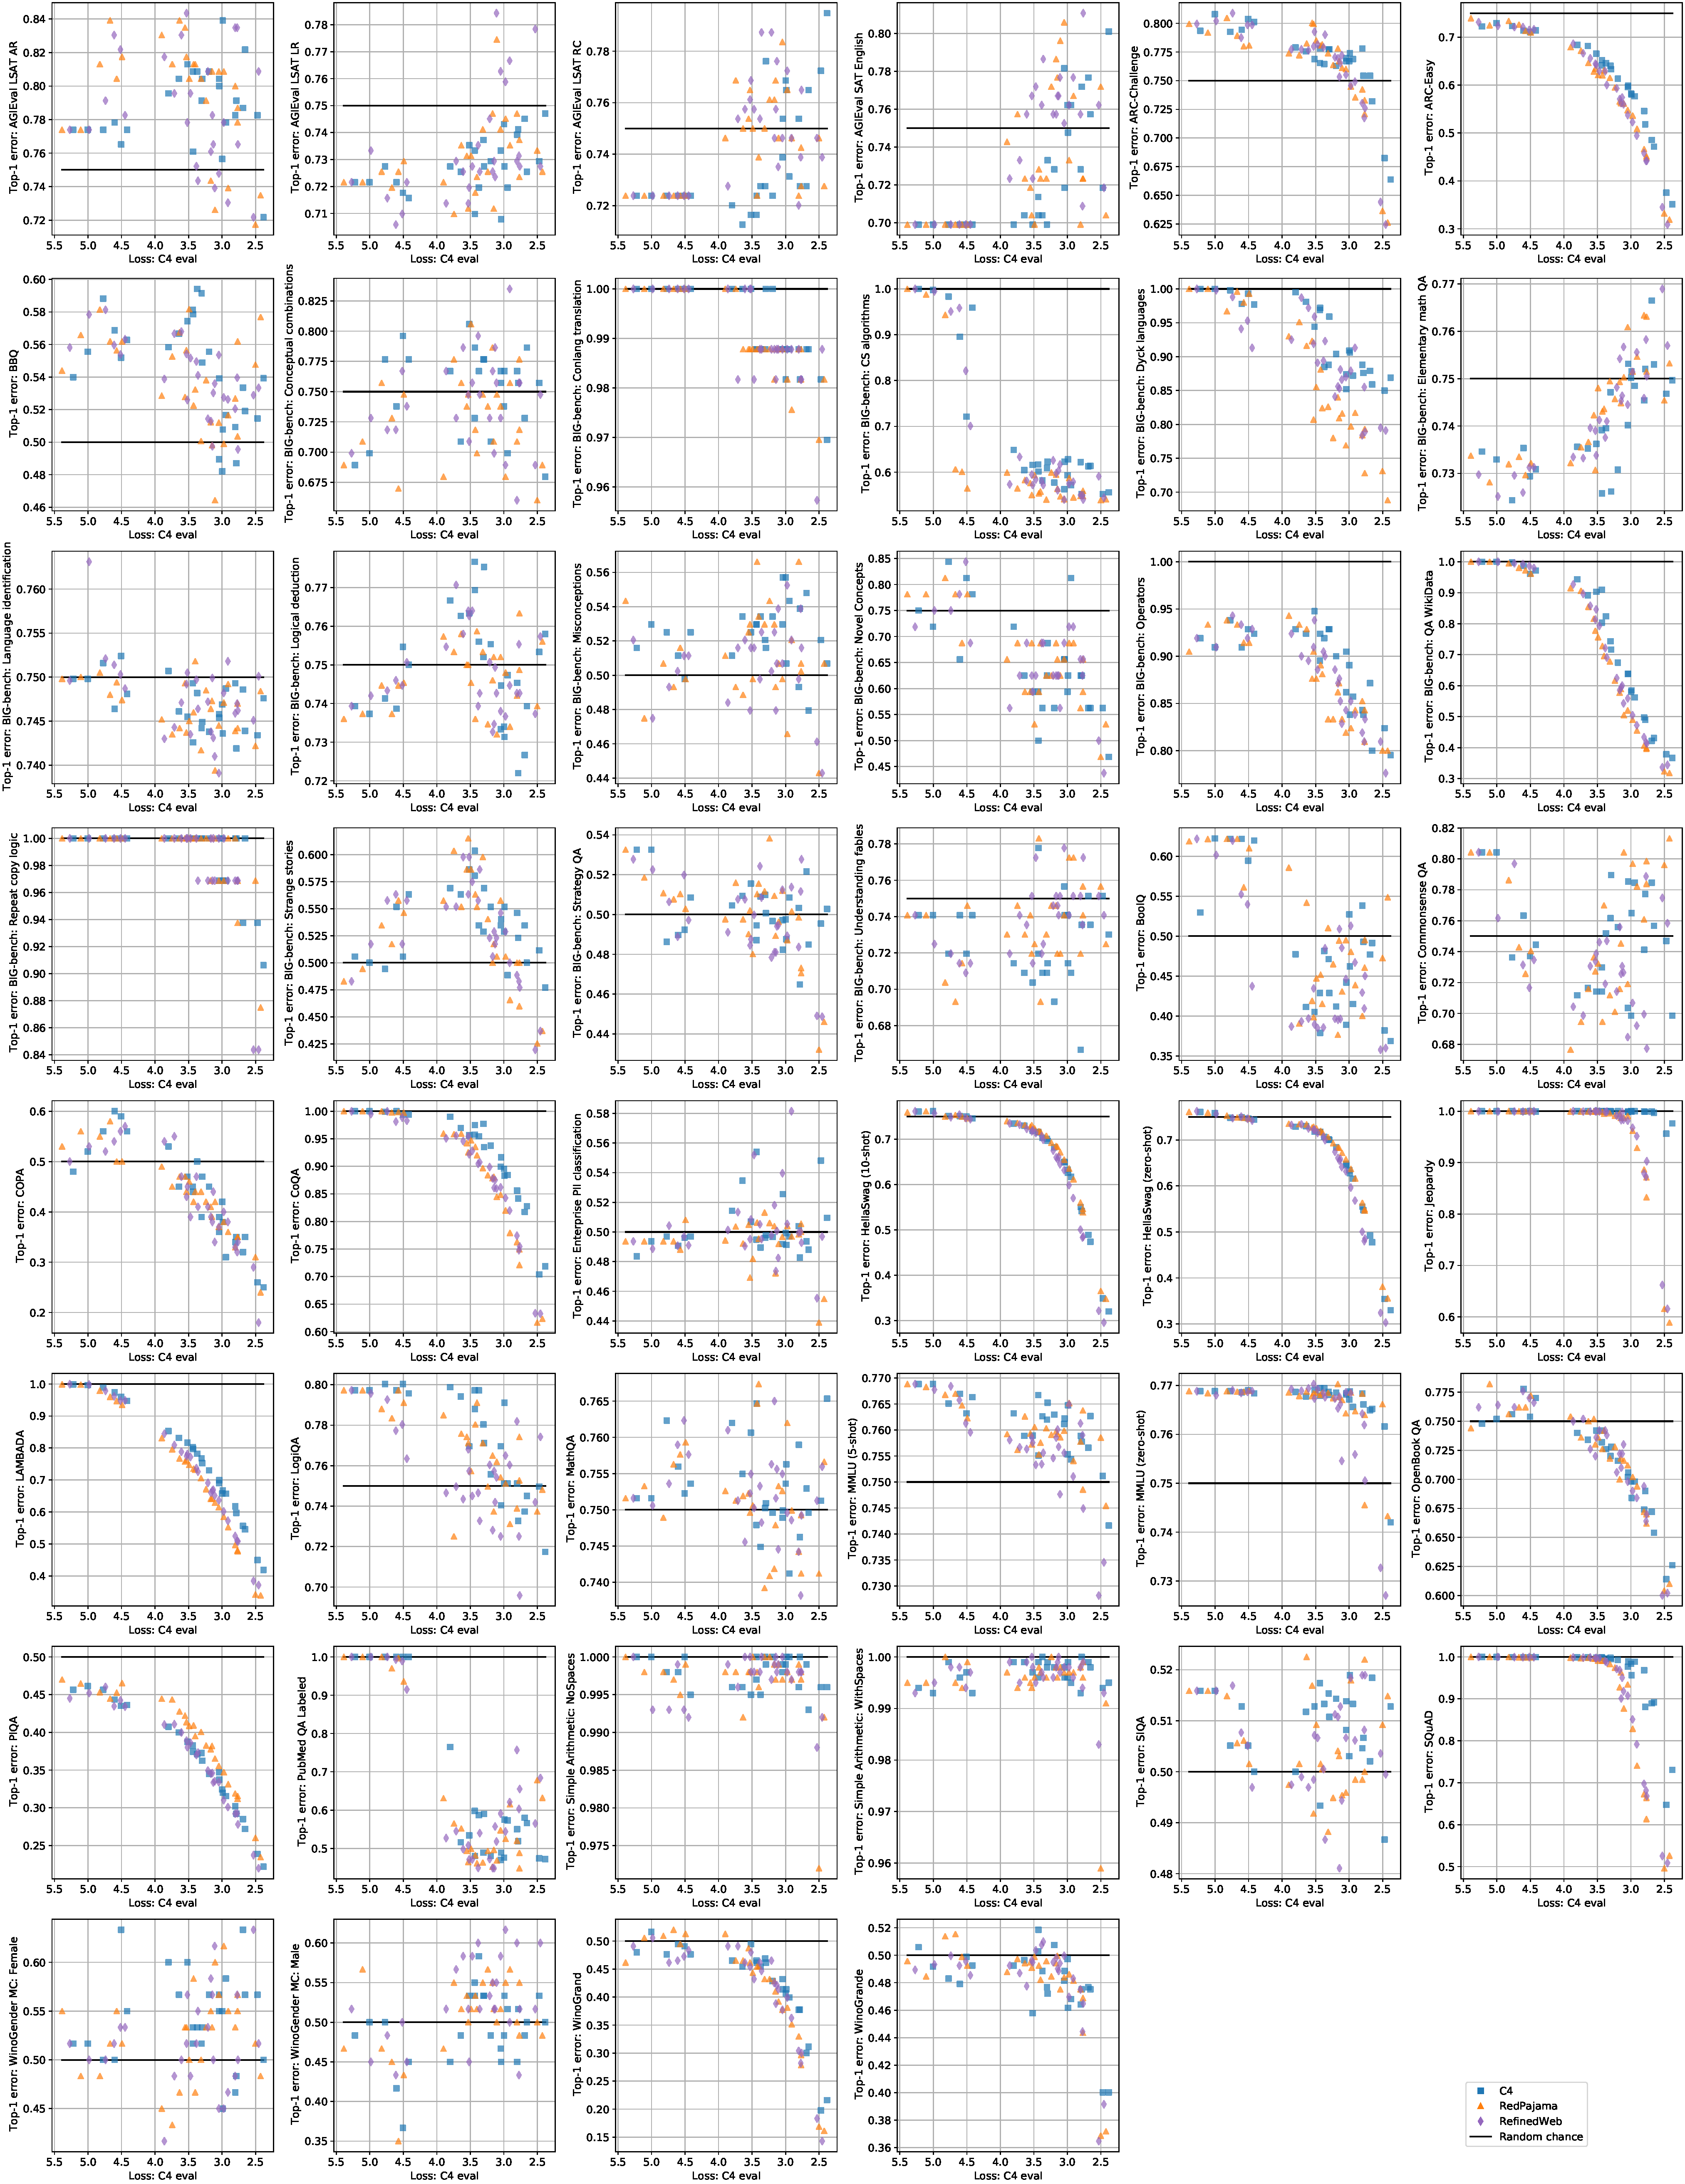
\includegraphics[width=0.9\textwidth]{figs/downstream_corr_all.pdf}
    \caption{\textbf{Downstream top-1 error vs. C4 eval loss for each of the 46 downstream evals.} Here we plot models from our testbed for each scatter plot.
    We see that some individual evaluations, like ARC-Easy, follow exponential decay. Others, like BIG-bench: CS algorithms, show step function behavior. Still others, like MathQA, hover around random chance.}
    \label{fig:mega}
\end{figure}

\paragraph{On compute-optimal token multipliers.}
We consider 20 tokens per parameter as close to compute-optimal for our experiments.
Here we investigate, using different approaches, what the compute-optimal token multipliers are for each dataset---assuming one should scale number of parameter and training tokens equally as~\citet{chinchilla} suggest.

Turning to Figure~\ref{fig:emperical_small}, we notice that there are many multipliers, between 10 and 80 that yield models close to the frontier.
Hence, empirically, it appears choices within this range should be suitable for the optimal token multiplier.

We can also compute an optimal token multiplier using the coefficients in Table~\ref{tab:fits}.
Based on \citet{chinchilla}'s Equation (4) and the assumption that $\alpha=\beta$, we write,
\begin{align}
\label{eq:m1}
N^*(C) = G \left( \frac{C}{6} \right)^{\frac{1}{2}}, D^*(C) = G^{-1} \left( \frac{C}{6} \right)^{\frac{1}{2}}, G = \left( \frac{a}{b}\right)^{\frac{1}{4\eta}}.
\end{align}
To compute $M^* = D^*/N^*$, we then have,
\begin{align}
\label{eq:m2}
M^* = \left( \frac{b}{a}\right)^{\frac{1}{2\eta}}.
\end{align}
Using the values from Table~\ref{tab:fits} and Equation~\eqref{eq:m2}, we find $M^*_{\text{C4}}=3.36$, $M^*_{\text{RedPajama}}=7.42$, $M^*_{\text{RefinedWeb}}=5.85$, where the subscript gives the dataset name.
These values conflict with the observation in Figure~\ref{fig:emperical_small}, which suggests $M=5$ is already too small to give points on the Pareto frontier.
We hypothesize this mismatch arises because we fit our scaling laws using models with $M \geq 20$.
Additionally, we hyperparamter-tune at $M=20$.
As previously discussed, it is likely possible to find better hyperparameter configurations at $M=5$ with further hyperparameter tuning at this token multiplier.

\section{Additional related work}
\label{appx:added_related}

\paragraph{Language modeling.}
Language models can be grouped into encoder-only~\cite{devlin-etal-2019-bert,albert,roberta,Sanh2019DistilBERTAD,clark2020electra}, encoder-decoder~\cite{lewis-etal-2020-bart,raffel2020exploring}, and decoder-only architectures~\cite{Radford2019LanguageMA,llama,llama2,MosaicML2023Introducing,jiang2023mistral,gunasekar2023textbooks,XGen,artetxe-etal-2022-efficient,thoppilan2022lamda,du2022glam,luukkonen2023fingpt,scao2022language,workshop2022bloom,allal2023santacoder,li2023starcoder,lozhkov2024starcoder,groeneveld2024olmo}.
Most current implementations are based on the transformer~\cite{transformer}. However, there has been a recent resurgence in scaling language models based on non-transformer architectures~\cite{peng-etal-2023-rwkv,gu2021combining,gu2021efficiently,mamba}.
Further, there has been substantial work on adapting pre-trained language models to better follow instructions~\cite{wei2021finetuned,chung2022scaling,muennighoff2022crosslingual,longpre2023data,muennighoff2023octopack,zhuo2024astraios,rafailov2024direct,ethayarajh2024kto,ustun2024aya,singh2024aya,muennighoff2024generative}.
However, following prior work~\cite{chinchilla,muennighoff2023scaling} and given their overall prevalence, we limit ourselves to GPT-style, decoder-only transformers that have solely been pre-trained.

\paragraph{Scaling laws.}
\citet{kaplan2020scaling} investigate scaling trends in GPT language models. 
\citet{bahri2021explaining} investigate different scaling regimes theoretically, and \citet{sharma_ScalingLawsData_2022} relate scaling coefficients to data manifold dimensions.
\citet{tay2021scale,tay-etal-2023-scaling} elucidate the connection between model architecture and scaling trends, while \citet{Hernandez2021ScalingLF,tay2021scale} develop scaling laws for transfer learning.
\citet{ivgi2022scaling} also consider transfer learning scaling laws and highlight the importance of hyperparameter selection in the low-compute regime.
\citet{ghorbani2021scaling,gordon-etal-2021-data,bansal2022data} develop scaling laws for neural machine translation.
\citet{caballero2023broken} propose a scaling law functional form, which they demonstrate is predictive in several domains.

\paragraph{Scaling beyond language modeling.}
There is a large body of work on scaling neural networks beyond language modeling, for example in computer vision~\cite{liu2022convnet,zhai2022scaling,sorscher2022beyond,abnar2022exploring,alabdulmohsin2022revisiting}, multimodal learning~\cite{Henighan2020ScalingLF,cherti2023reproducible,datacomp}, and image reconstruction~\cite{klug2023analyzing}. 

\paragraph{Over-training in existing models.}
%!TEX root = ../main.tex

\section{Related Work}
\label{sec:related}

\textbf{State space models} have shown promise in modeling sequential data, including time series data~\citep{gu2022efficiently}, audio~\citep{goel2022s}, and visual data~\citep{nguyen2022s4nd}.
Our model builds off work on simplifying and parameterizing diagonal versions of S4~\citep{gu2022parameterization,gupta2022diagonal, gu2022train}.
Gated state spaces~\citep{mehta2022long} also aim to adapt SSMs to language modeling, but our results suggest that the GSS model does not perform as well as \hthree (or even as well as earlier SSMs like S4D).
The idea to combine SSMs with attention in hybrid models is not new; Mehta et al.~\citep{mehta2022long} also showed that interleaving attention with their GSS layer can improve performance, which we also validate on our OpenWebText experiments.
These positive results suggest that attention and SSMs are complementary, and that hybrid models may be a promising direction for future work.

\textbf{Large language foundation models}~\citep{bommasani2021opportunities} have demonstrated the power of scaling attention-based networks to billions of parameters and training them on trillions of tokens~\citep{hoffmann2022training}.
Understanding the mechanistic basis~\citep{elhage2021mathematical} behind these models may yield insights into better design choices for future models.
These and similar explorations have informed the design of \hthree and our selection of synthetic languages.
A number of recent works have also explored how to address the shortcomings of attention by approximating the attention computation~\citep{wang2020linformer,katharopoulos2020transformers, choromanski2020rethinking,tay2020long, kitaev2020reformer, daras2020smyrf}.
We believe these efforts are complementary to SSMs, and we are excited to see how they can be combined in future work.

\textbf{Linear attention}~\citep{katharopoulos2020transformers} and classical sequence models like RNNs serve as inspiration for \hthree.
Appendix~\ref{app:linear_attention} draws a direct connection between linear attention and LTI systems.
Luo et al.~\citep{luo2021stable} also propose a variant of linear attention that can achieve $O(n \log n)$ scaling in sequence length.
Appendix~\ref{sec:app_additional_experiments} evaluates linear attention on language modeling, and finds that it underperforms exact attention, whereas \hthree outperforms attention.
The multiplicative interactions in \hthree are reminiscent of gating mechanisms in LSTMs~\citep{hochreiter1996lstm} and GRUs~\citep{cho2014properties}, which suggests that architectural lessons from these sequence models may be useful for adapting SSMs to language modeling.
A number of algorithms for scaling attention to longer sequences have also been proposed, such as Transformer-XL~\citep{dai2019transformer}, Reformer~\citep{kitaev2020reformer}, Performer~\citep{choromanski2020rethinking}, and Perceiver AR~\citep{hawthorne2022general}.
Some of these approaches underperform exact attention on language modeling, and may be slower in wall-clock speed~\citep{dao2022flashattention}.
A thorough comparison of these alternatives to exact attention and how well they scale in model size and amount of training data is fruitful future work.

\textbf{FFT} algorithms are used in a wide variety of applications, including signal processing~\citep{oppenheim1978applications}, control theory~\citep{brogan1974modern}, and more.
Various algorithms for computing the FFT have existed for decades~\citep{oppenheim2001discrete}.
We hope our work on appealing to these classic algorithms to accelerate new applications such as learned SSMs will inspire future algorithmic exploration, even if hardware is not designed for them~\citep{hooker2021hardware}.

%%% Local Variables:
%%% mode: latex
%%% TeX-master: "../main"
%%% End:

To contextualize the extent to which we over-train, we provide token multipliers for popular models in Table~\ref{tab:other_mults}.

\section{Broader impact}
\label{appx:broader}

Language models have known risks in terms of harmful language, toxicity, and human automation---to name a few~\cite{weidinger2021ethical,bender2021dangers}.
We include the following for our public release ``WARNING: These are base models and not aligned with post-training. They are provided as is and intended as research artifacts only.''
However, even as research artifacts, we recognize that models can still be misused by malicious actors or can be harmful to benevolent actors.
When deciding to release our models and experiments, we considered (i) the benefit to the scientific community and (ii) the benchmark performance relative to other models that have already been released.
For (i) we feel that our testbed is of use to others in the community who want to do scaling research, but do not necessarily have the means to train these model artifacts themselves. Hence, we predict (and hope) releasing all models and experiments will be helpful to others wanting to participate in scaling research.
For (ii), we note that there are publicly available models~\cite{llama,llama2,jiang2023mistral}, which outperform models from our testbed and that are more likely to be widely adopted.
Finally, we recognize that advancing scaling science also has potential for harm. Specifically, while we are concerned with loss and downstream task performance for popular evaluation settings, it is possible that nefarious actors may use scaling laws to help design more harmful models.

\end{appendix}